%!TEX root = ../FundationsDataScience.tex

\chapter{Machine Learning}


% Refs \cite{rosasco2017notes,friedman2001elements,murphy2012machine}

This chapter gives a rapid overview of the main concepts in machine learning. The goal is not to be exhaustive, but to highlight representative problems and insist on the distinction between unsupervised (vizualization and clustering) and supervised (regression and classification) setups. We also shed light on the tight connexions between machine learning and inverse problems.

While imaging science problems are generally concern with processing a single data (e.g. an image), machine learning problem is rather concern with analysing large collection of data. The focus (goal and performance measures) is thus radically different, but quite surprisingly, it uses very similar tools and algorithm (in particular linear models and convex optimization). 


%%%%%%%%%%%%%%%%%%%%%%%%%%%%%%%%%%%%%%%%%%%%%%%%%%
%%%%%%%%%%%%%%%%%%%%%%%%%%%%%%%%%%%%%%%%%%%%%%%%%%
%%%%%%%%%%%%%%%%%%%%%%%%%%%%%%%%%%%%%%%%%%%%%%%%%%
\section{Unsupervised Learning}

In unsupervised learning setups, one observes $n$ points $(x_i)_{i=1}^n$. 
%
The problem is now to infer some properties for this points, typically for vizualization or unsupervised classication (often called clustering). 
%
For simplicity, we assume the data are points in Euclidean space $x_i \in \RR^p$ ($p$ is the so-called number of features). These points are conveniently stored as the rows of a matrix $X \in \RR^{n \times d}$.


%%%%%%%%%%%%%%%%%%%%%%%%%%%%%%%%%%%%%%%%%%%%%%%%%%
\subsection{Dimensionality Reduction and PCA}

Dimensionality reduction is useful for vizualization. It can also be understood as the problem of feature extraction (determining which are the relevant parameters) and this can be later used for doing other tasks more efficiently (faster and/or with better performances). 
%
The simplest method is the Principal Component Analysis (PCA),  which performs an orthogonal linear projection on the principal axes (eigenvectors) of the covariance matrix.

%%%
\paragraph{Presentation of the method.}

The empirical mean is defined as 
\eq{
    \hat m \eqdef \frac{1}{n} \sum_{i=1}^n x_i \in \RR^p
} 
and  covariance
\eql{\label{eq-emp-cov}
 	\hat C \eqdef \frac{1}{n} \sum_{i=1}^n (x_i-\hat m) (x_i-\hat m)^* \in \RR^{p \times p}. 
}
Denoting $\tilde X \eqdef X - 1_p \hat m^*$, one has $\hat C=\tilde X^*
\tilde X/n$. 

Note that if the points $(x_i)_i$ are modelled as i.i.d. variables, and denoting $\xp$ one of these random variables, one has, using the law of large numbers, the almost sure convergence as $n \rightarrow +\infty$
\eql{\label{eq-cov-approx}
	\hat m \rightarrow m \eqdef \EE(\xp)
	\qandq
	\hat C \rightarrow C \eqdef \EE((\xp-m)(\xp-m)^*).
}
Denoting $\mu$ the distribution (Radon measure) on $\RR^p$ of $\xp$, one can alternatively write
\eq{
	m = \int_{\RR^p} x \d\mu(x)
	\qandq
	C = \int_{\RR^p} (x-m)(x-m)^* \d\mu(x).	
}


\begin{figure}
\centering
\begin{tabular}{@{}c@{}c@{}}
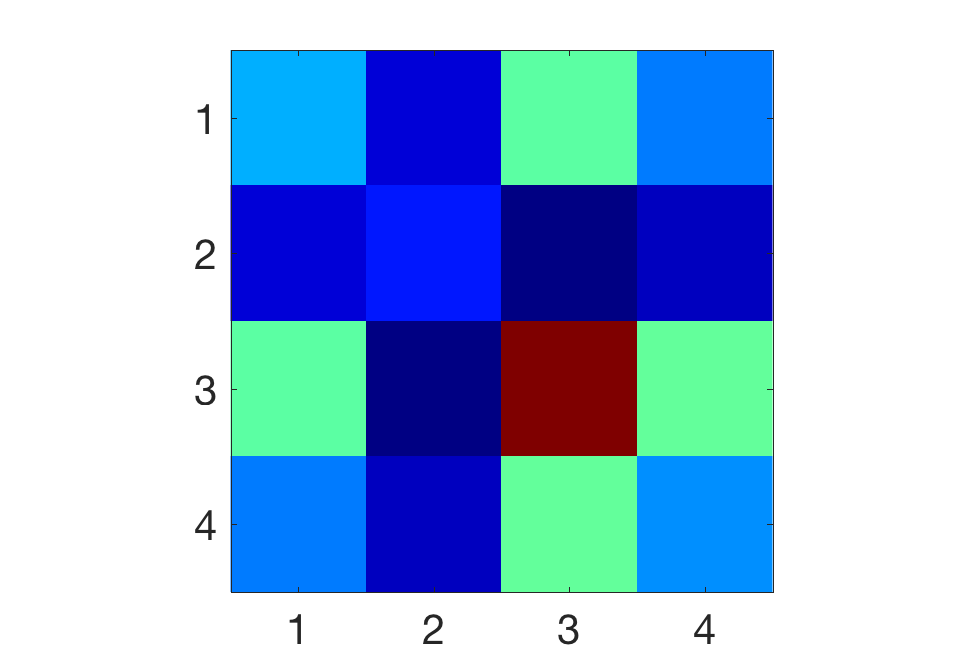
\includegraphics[width=.25\linewidth]{ml/pca-nn/cov}&
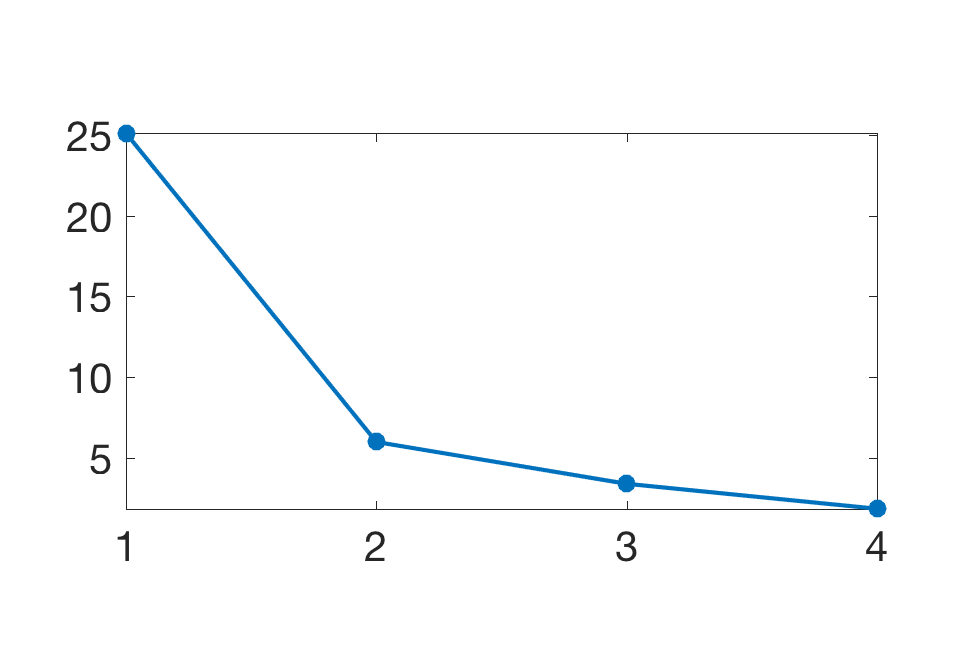
\includegraphics[width=.4\linewidth]{ml/pca-nn/svd}\\
$C$ & SVD of $C$
\end{tabular}
\caption{\label{fig-cov}
Empirical covariance of the data and its associated singular values. 
}
\end{figure}


\wrapf{ml/variance}{PCA main axes capture variance}
The PCA ortho-basis, already introduced in Section~\ref{prop-svd}, corresponds to the right singular vectors of the centred data matrix, as defined using the (reduced) SVD decomposition
\eq{
 	\tilde X = \sqrt{n} U \diag(\si) V^*
}
where $U \in \RR^{n \times r}$ and $V \in \RR^{p \times r}$, and where $r=\rank(\tilde X) \leq \min(n,p)$. 
%
We denote $V=(v_k)_{k=1}^r$ the orthogonal columns (which forms an orthogonal system of eigenvectors of $\hat C = V \diag(\si^2) V^\top$), $v_k \in \RR^p$. The intuition is that they are the main axes of ``gravity'' of the point cloud  $(x_i)_i$ in $\RR^p$.
%
We assume the singular values are ordered, $\si_1 \geq \ldots \geq \si_r$, so that the first singular values capture most of the variance of the data. 

Figure~\ref{fig-cov} displays an example of covariance and its associated spectrum $\si$. The points $(x_i)_i$ correspond to the celebrated
IRIS dataset\footnote{\url{https://en.wikipedia.org/wiki/Iris_flower_data_set}} of Fisher. This dataset consists of 50 samples from each of three species of Iris (Iris setosa, Iris virginica and Iris versicolor). The dimensionality of the features is $p=4$, and the dimensions corresponds to the length and the width of the sepals and petals. 

The PCA dimensionality reduction embedding $x_i \in \RR^p \mapsto z_i \in \RR^d$ in dimension $d \leq p$ is obtained by projecting the data on the first $d$ singular vector
\eql{\label{eq-pca-1}
	z_i \eqdef ( \dotp{x_i-m}{v_k} )_{k=1}^d \in \RR^d. 
}
From these low-dimensional embedding, one can reconstruct back an approximation as
\eql{\label{eq-pca-2}
	\tilde x_i \eqdef m+\sum_k z_{i,k} v_k \in \RR^p.
}
One has that $\tilde x_i = \Proj_{\tilde T}(x_i)$ where $\tilde T \eqdef m + \Span_{k=1}^d(v_k)$ is an affine space.

Figure~\ref{fig-pca} shows an example of PCA for 2-D and 3-D vizualization.

\begin{figure}
\centering
\begin{tabular}{@{}c@{\hspace{5mm}}c@{}}
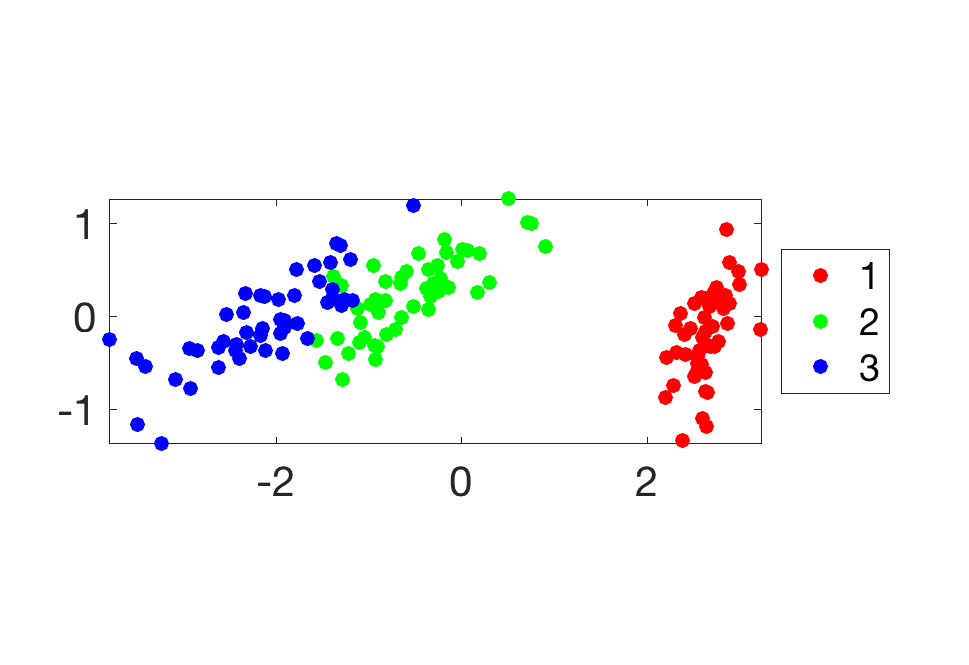
\includegraphics[width=.4\linewidth]{ml/pca-nn/points-2d}&
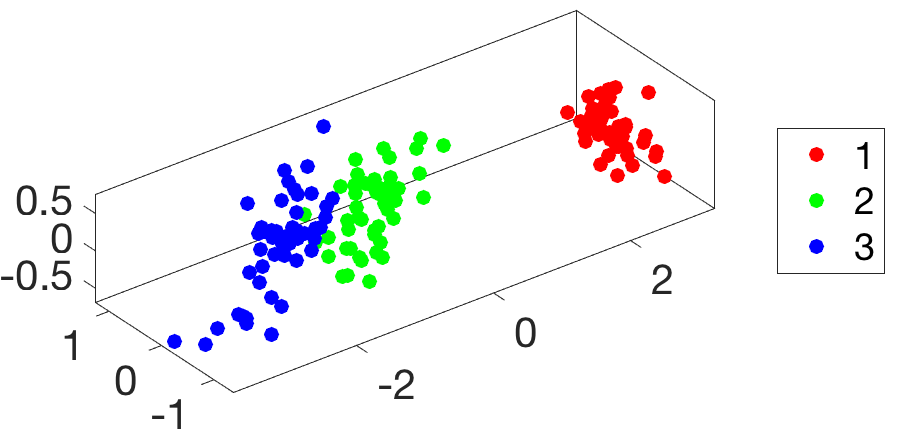
\includegraphics[width=.4\linewidth]{ml/pca-nn/points-3d}
\end{tabular}
\caption{\label{fig-pca}
2-D and 3-D PCA vizualization of the input clouds. 
}
\end{figure}


%%%
\paragraph{Optimality analysis.}

\wrapfSimple{ml/pca-maths/pca-maths-1}
We now show that among all possible linear dimensionality reduction method, PCA is optimal in sense of $\ell^2$ error. 
%
To simplify, without loss of generality (since it can be subtracted from the data) we assume that empirical mean is zero $\hat m=0$ so that $X=\tilde X$. 

We recall that $X=\sqrt{n} U \diag(\si) V^\top$ and $\hat C = \frac{1}{n} X^\top X = U \La U^\top$ where $\La = \diag(\la_i=\si_i^2)$, where $\la_1 \geq \ldots \geq \la_r$.  

\wrapfSimple{ml/pca-maths/pca-maths-2}
The following proposition shows that PCA is optimal in term of $\ell^2$ distance if one consider only affine spaces. This means that we consider the following compression/decompression to a dimension $k$ (i.e. dimensionality reduction and then expansion) 
\eql{\label{eq-pca-nonconvex}
	\umin{R,S} \enscond{
		f(R,S) \eqdef \sum_i \norm{x_i-R S^\top x_i}_{\RR^p}^2
		}{ R,S \in \RR^{p \times k} }
}
Note that this minimization is a priori not trivial to solve because, although $f(\cdot,S)$ and $f(R,\cdot)$ are convex, $f$ is not jointly convex. So iteratively minimizing on $R$ and $S$ might fail to converge to a global minimizer.
%
This section aims at proving the following theorem.

\begin{thm}\label{thm-pca-optim}
	A solution of~\eqref{eq-pca-nonconvex} is $S=R=V_{1:k} \eqdef [v_1,\ldots,v_k]$.
\end{thm}

Note that using such a compressor $R$ and decompressor $R=S$ corresponds exactly to the PCA method~\eqref{eq-pca-1} and~\eqref{eq-pca-2}.

We first prove that one can restrain its attention to orthogonal projection matrix.

\begin{lem}
	One can assume $S=R$ and $S^\top S = \Id_{k\times k}$.
\end{lem}
\begin{proof}
	We consider an arbitrary pair $(R,S)$. Since the matrix $R S^\top$ has rank $k' \leq k$, let $W \in \RR^{p \times k'}$ be an ortho-basis of $\Im(RS^\top)$, so that $W^\top W = \Id_{k' \times k'}$. We remark that 
	\eq{
		\uargmin{z} \norm{x-Wz}^2 = W^\top x
	}
	because the first order condition for this problem reads $W^\top(Wz-x)=0$.
	%	
	Hence, denoting $RS^\top x_i = Wz_i$ for some $z_i \in \RR^{k'}$
	\eq{
		f(R,S) = \sum_i \norm{x_i - RS^\top x_i}^2 = \sum_i \norm{x_i - W z_i}^2 \geq \sum_i \norm{x_i - W W^\top x_i}^2
		\geq  f(\tilde W,\tilde W).
	}
	were we have extended $W$ in an orthogonal matrix $\tilde W \in \RR^{p \times k}$ where $\tilde W_{1:k'}=W$.
\end{proof}

\begin{lem}
	Denoting $C \eqdef XX^\top \in \RR^{p \times p}$, an optimal $S$ is obtained by solving
	\eq{
		\umax{S \in \RR^{p \times k}} \enscond{\tr(S^\top C S^\top)}{ S^\top S=\Id_{k} }.
	}
\end{lem}
\begin{proof}
	Using the previous lemma, one can consider only $R=S$ with $S^\top S=\Id_{k}$ so that one needs to solve
	\eq{
		f(S,S) = \sum_i \norm{x_i SS^\top x_i}^2
		= \sum_i \norm{x_i}^2 - 2 x_i^\top S S^\top x_i + x_i^\top S(S^\top S) S^\top x_i.
	}
	Using that $S^\top S=\Id_k$, one has
	\eq{
		f(S,S) = \text{cst} - \sum_i x_i^\top S S^\top x_i
		= - \sum_i \tr(x_i^\top S S^\top x_i)
		= - \sum_i \tr(S^\top x_i x_i^\top S )
		= - \tr( S^\top (\sum_i x_i x_i^\top) S ).
	}
\end{proof}

The next lemma provides an upper bound on the quantity being minimized as the solution of a convex optimization problem (a linear program). The proof of the theorem follows by showing that this upper bound is actually reached, which provides a certificate of optimality.  

\begin{lem}\label{lem-upper-bound-pca}
	Denoting $C=V \La V^\top$, one has 
	\eql{\label{eq-variational-pca}
		\tr(S^\top C S) \leq \umax{\be \in \RR^p}
			\enscond{ \sum_{i=1}^p \la_i \be_i }{ 0 \leq \be \leq 1, \sum_i \be_i \leq k }
			= \sum_{i=1}^k \la_i
	}
	i.e. the maximum on the right hand size is $\be=(1,\ldots,1,0,\ldots,0)$.
\end{lem}
\begin{proof}
	We extend $V \in \RR^{p \times k}$ into an orthogonal matrix $\tilde V \in \RR^{p \times p}$ (i.e. $\tilde V_{1:r}=V$) such 
	that $\tilde V\tilde V^\top = \tilde V^\top V = \Id_p$. Similarly we extend $\La$ into $\tilde\La$ by adding zeros, so that $C=\tilde V \tilde \La \tilde V^\top$.  One has
	\eq{
		\tr(S^\top C S) = \tr(S^\top \tilde V \tilde \La \tilde V^\top S)
		= \tr(B^\top \La B) = \tr(\La BB^\top) = \sum_{i=1}^p \la_i \norm{b_i}^2
		= \sum_i \la_i \be_i
	}
	where we denoted $B \eqdef V^\top S \in \RR^{p \times k}$, $(b_i)_{i=1}^p$ with $b_i \in \RR^k$ are the rows of $B$ and $\be_i \eqdef \norm{b_i}^2 \geq 0$.
	%
	One has
	\eq{
		B^\top B = S^\top \tilde V \tilde V^\top S = S^\top S = \Id_k, 
	}
	so that the columns of $B$ are orthogonal, and thus
	\eq{
		\sum_i \be_i = \sum_i \norm{b_i}^2 = \norm{B}_{\text{Fro}}^2 = \tr(B^\top B) = \tr(B^\top B) = k.
	}		
	
	\begin{figure}
\centering
\begin{tabular}{@{}c@{\hspace{10mm}}c@{\hspace{10mm}}c@{}}
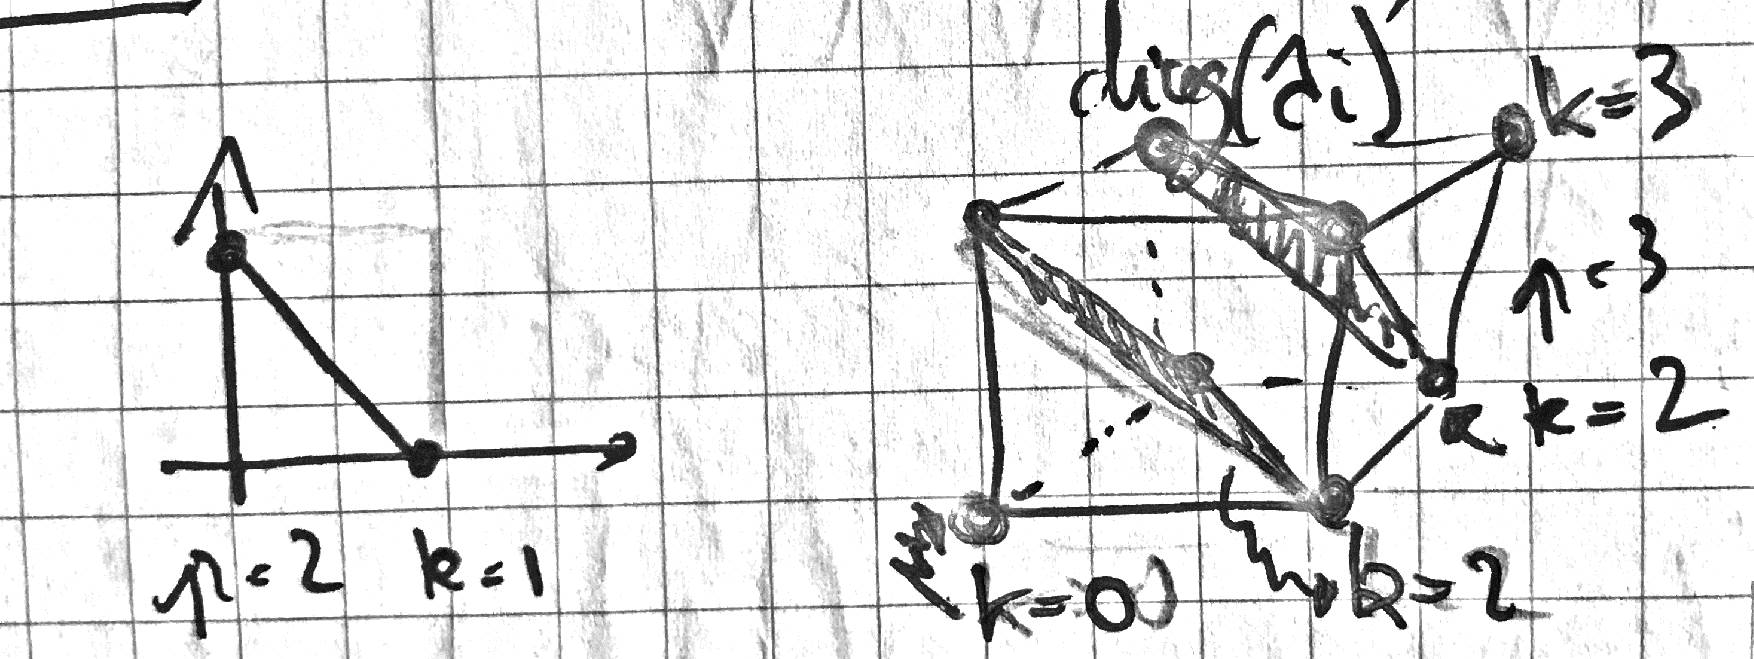
\includegraphics[width=.3\linewidth]{ml/pca-maths/pca-maths-3}&
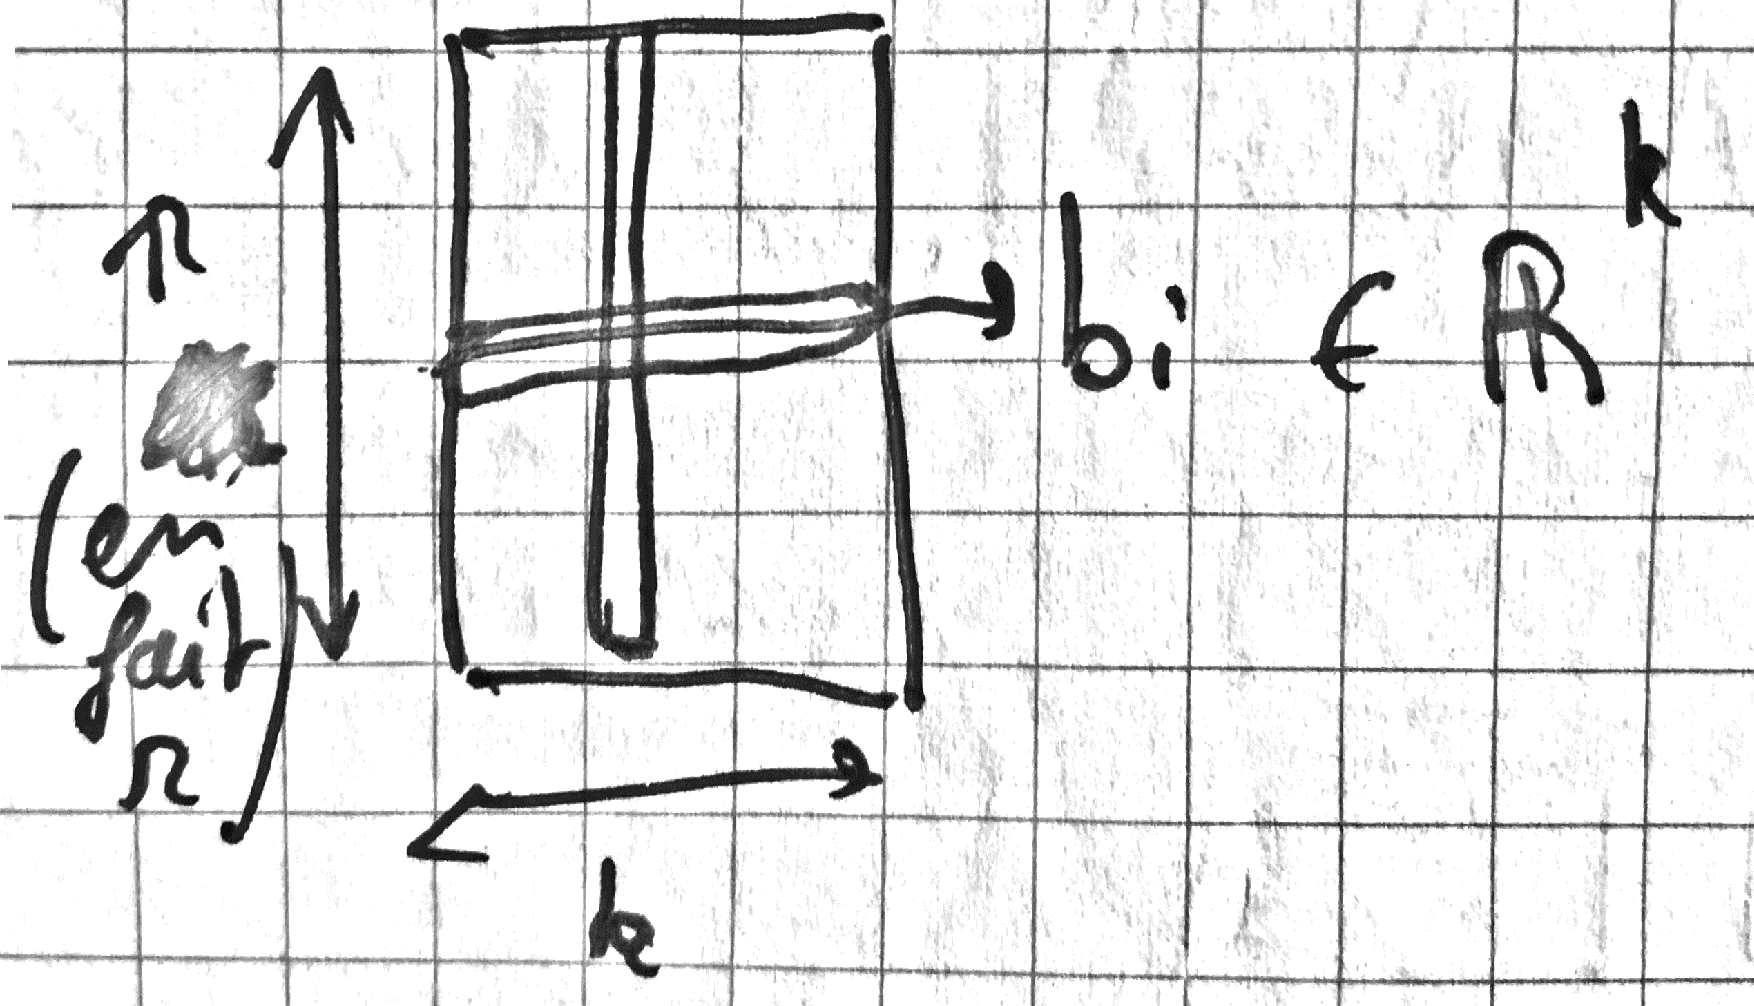
\includegraphics[width=.2\linewidth]{ml/pca-maths/pca-maths-4}&
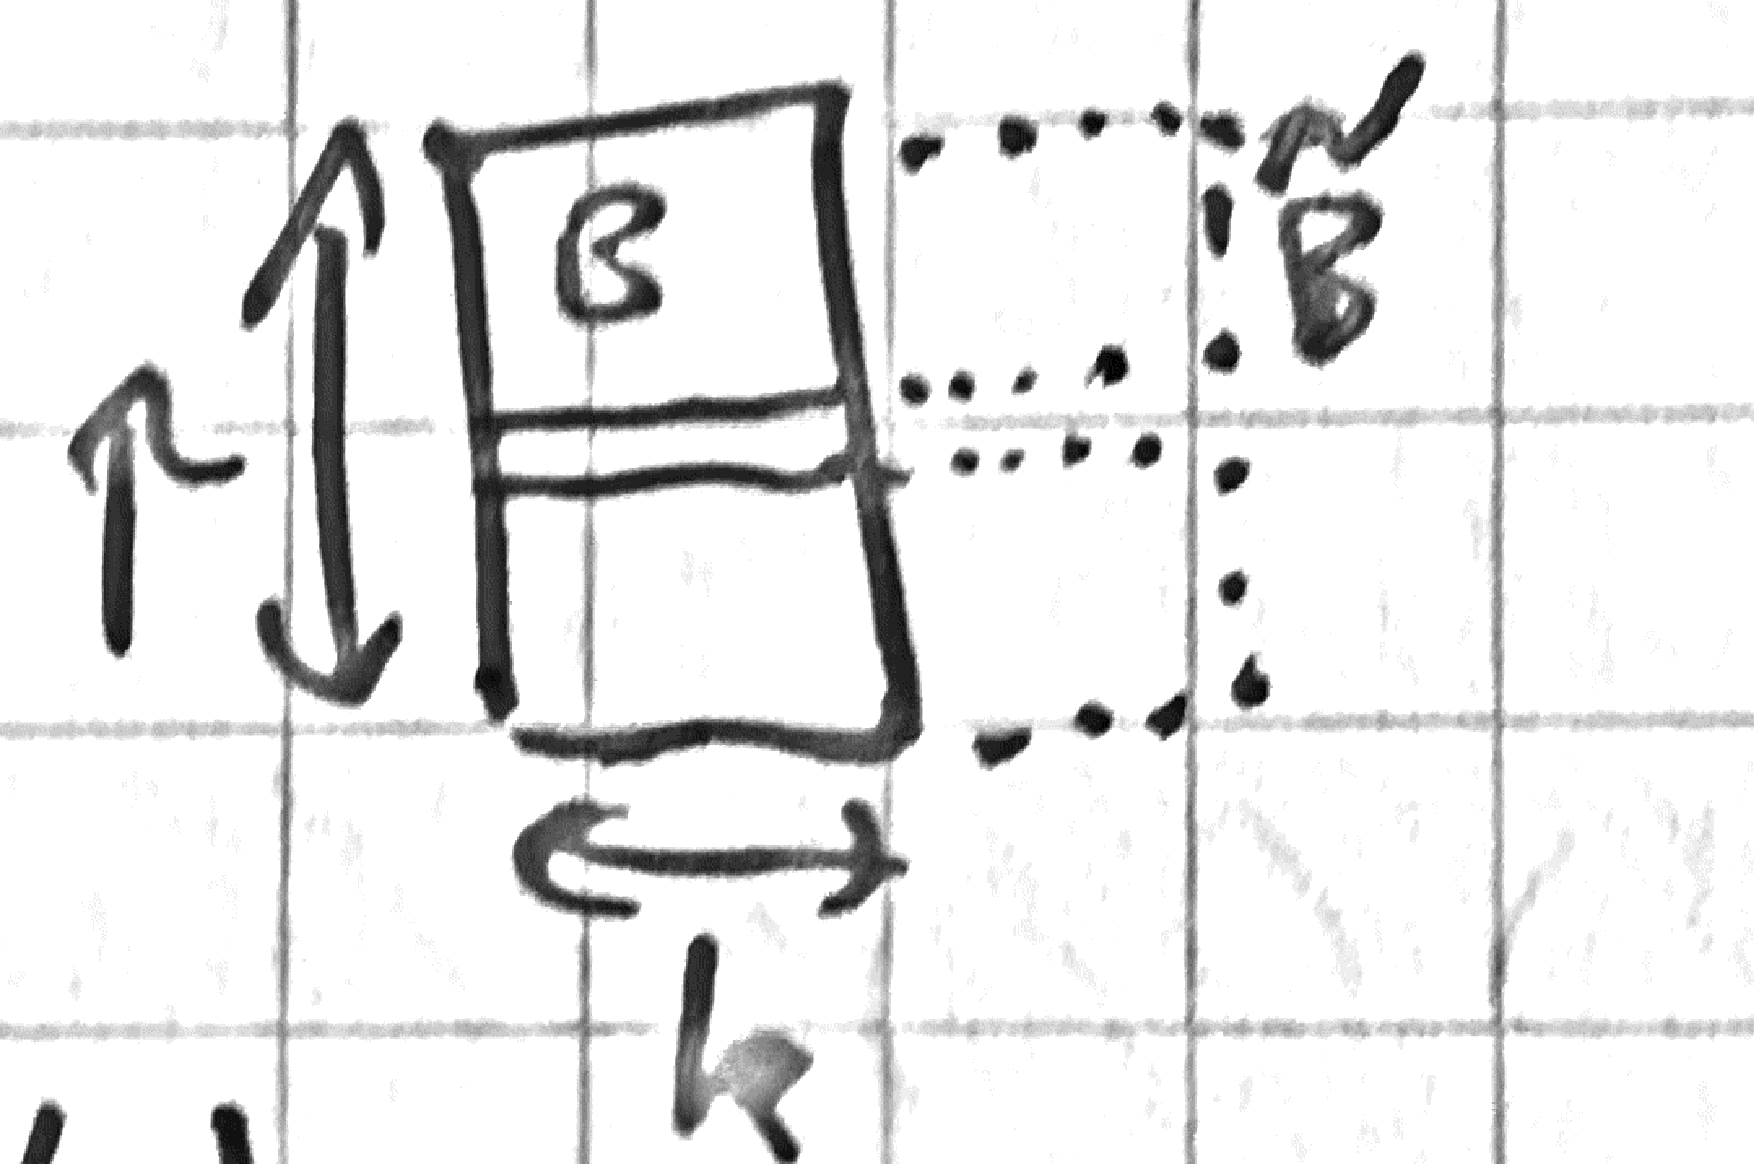
\includegraphics[width=.2\linewidth]{ml/pca-maths/pca-maths-5}
\end{tabular}
\caption{\label{fig-pca-var-proof}
Left: proof of the rightmost inequality in~\eqref{eq-variational-pca}. Middle: matrix $B$, right: matrix $\tilde B$. 
}
\end{figure}


	We extend the $k$ columns of $b$ into an orthogonal basis $\tilde B \in \RR^{p \times p}$ such that $\tilde B \tilde B^\top = \tilde B^\top \tilde = \Id_p$, so that 
	\eq{
		0 \leq \be_i = \norm{b_i}^2 \leq \norm{\tilde b_i}^2 = 1
	}
	and hence $(\be_i)_{i=1}^p$ satisfies the constraint of the considered optimization problem, hence $\tr(S^\top C S)$ 
	is necessarily smaller than the maximum possible value. 
	%
	
	For the proof of the second upper bound, we only verify it in 2D and 3D using a drawing, see Figure~\ref{fig-pca-var-proof}, left. 
\end{proof}

\begin{proof}[Proof of Theorem~\ref{thm-pca-optim}]
	Setting $S=V_{1:k}=[v_1,\ldots,v_k]$, it satisfies $CS = V \La V^\top V_{1:k} = V_{1:k} \diag(\la_i)_{i=1}^k$ and hence
	\eq{
		\tr(S^\top C S) = \tr(S^\top S \diag(\la_i)_{i=1^k}) = \tr(\Id_k \diag(\la_i)_{i=1^k}) = \sum_{i=1}^k \la_i.
	}
	This value matches the right-most upper bound of Lemma~\ref{lem-upper-bound-pca}, which shows that this $S$ is optimal.
\end{proof}


%\begin{prop}
%	One has
%	\eq{
%		(\tilde x,\tilde T) \in \uargmin{ (\bar x,\bar T) } \enscond{ \sum_i \norm{x_i - \bar x_i }^2 }{ \foralls i, \bar x_i \in \bar T }
%	}
%	where $\bar T$ is constrained to be a $d$-dimensional affine space. 
%\end{prop}

 
 

%%%%%%%%%%%%%%%%%%%%%%%%%%%%%%%%%%%%%%%%%%%%%%%%%%%%%%%%%%%%%%%%%%
\subsection{Clustering and $k$-means}

A typical unsupervised learning task is to infer a class label $y_i \in \{1,\ldots,k\}$ for each input point $x_i$, and this is often called a clustering problem (since the set of points associated to a given label can be thought as a cluster).

%%%%
\paragraph{$k$-means}

A way to infer these labels is by assuming that the clusters are compact, and optimizing some compactness criterion. Assuming for simplicity that the data are in Euclidean space (which can be relaxed to an arbitrary metric space, although the computations become more complicated), the $k$-means approach minimizes the distance between the points and their class centroids $c=(c_\ell)_{\ell=1}^k$, where each $c_\ell \in \RR^p$. The corresponding variational problem becomes
\eq{
	\umin{ (y,c) } \Ee( y, c ) \eqdef \sum_{\ell=1}^k \sum_{ i : y_i=\ell } \norm{x_i-c_\ell}^2. 
}

\wrapf{ml/voronoi}{$k$-means clusters according to Vornoi cells.}
The $k$-means algorithm can be seen as a block coordinate relaxation, which alternatively updates the class labels and the centroids.
%
The centroids $c$ are first initialized (more on this later), for instance, using a well-spread set of points from the samples.  
% 
For a given set $c$ of centroids, minimizing $y \mapsto \Ee(y,c)$ is obtained in closed form by assigning as class label the index of the closest centroids
\eql{\label{eq-kmeans-1}
	\foralls i \in \{1,\ldots,n\}, \quad y_i \leftarrow \uargmin{1 \leq \ell \leq k} \norm{x_i-c_\ell}.
}
For a given set $y$ of labels, minimizing $c \mapsto \Ee(y,c)$ is obtained in closed form by computing the barycenter of each class
\eql{\label{eq-kmeans-2}
	\foralls \ell \in \{1,\ldots,k\}, \quad c_\ell \leftarrow \frac{
		\sum_{i : y_i=\ell} x_i
	}{
		|\enscond{i}{y_i=\ell}|
	}
}
If during the iterates, one of the cluster associated to some $c_\ell$ becomes empty, then one can either decide to destroy it and replace $k$ by $k-1$, or try to ``teleport'' the center $c_\ell$ to another location (this might increase the objective function $\Ee$ however). 

Since the energy $\Ee$ is decaying during each of these two steps, it is converging to some limit value. Since there is a finite number of possible labels assignments, it is actually constant after a finite number of iterations, and the algorithm stops. 

Of course, since the energy is non-convex, little can be said about the property of the clusters output by $k$-means.
%
To try to reach lower energy level, it is possible to ``teleport'' during the iterations centroids $c_\ell$ associated to clusters with high energy to locations within clusters with lower energy (because optimal solutions should somehow balance the energy).  

Figure~\ref{fig-kmeans} shows an example of $k$-means iterations on the Iris dataset.

\begin{figure}
\centering
\begin{tabular}{@{}c@{\hspace{10mm}}c@{}}
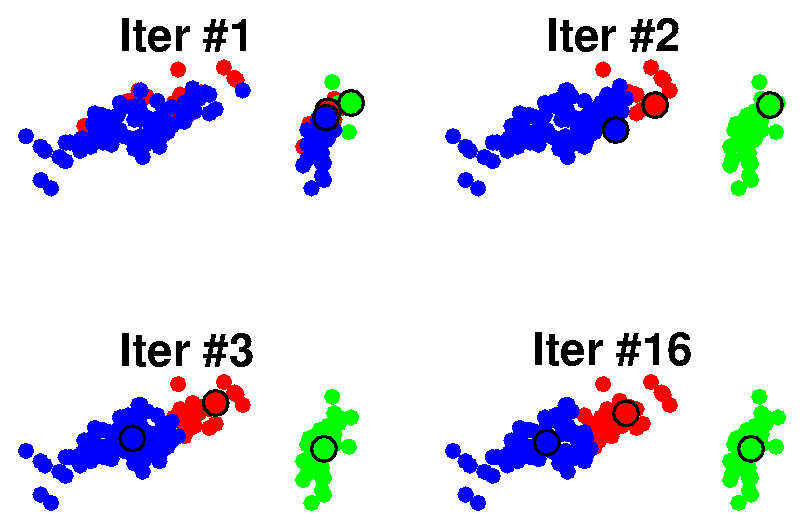
\includegraphics[width=.4\linewidth]{ml/pca-nn/kmeans-iter}&
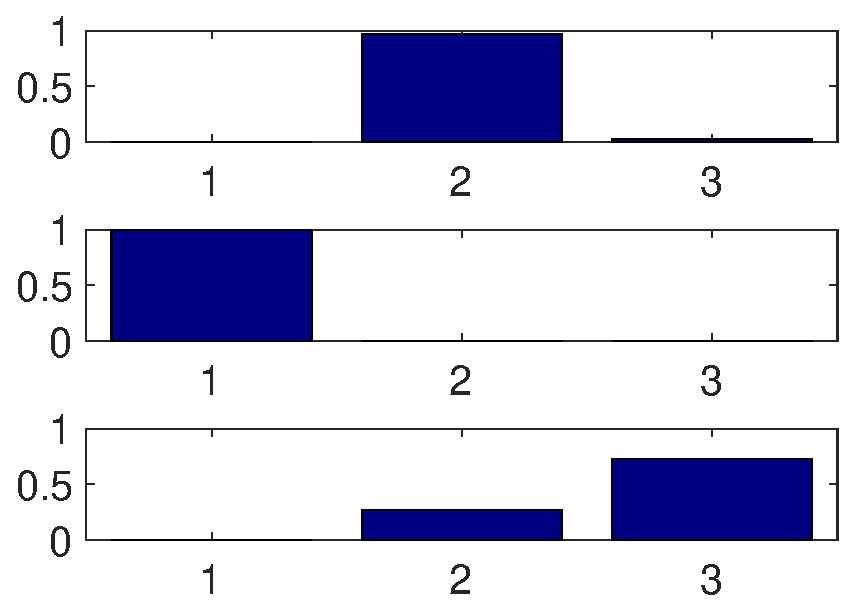
\includegraphics[width=.35\linewidth]{ml/pca-nn/kmeans-classif-scores}
\end{tabular}
\caption{\label{fig-kmeans}
Left: iteration of $k$-means algorithm. Right: histogram of points belonging to each class after the $k$-means optimization. 
}
\end{figure}


%%%%
\paragraph{$k$-means++}

To obtain good results when using $k$-means, it is crucial to have an efficient initialization scheme. In practice, the best results are obtained by seeding them as far as possible from one another (a greedy strategy works great in practice). 

Quite surprisingly, there exists a randomized seeding strategy which can be shown to be close to optimal in term of value of $\Ee$, even without running the $k$-means iterations (although in practice it still needs to be used to polish the results). The corresponding $k$-means++ initialization is obtained by selecting $c_1$ uniformly at random among the $x_{i}$, and then assuming $c_\ell$ has been seeded, drawing $c_{\ell+1}$ among the sample according to the probability $\pi^{(\ell)}$ on $\{1,\ldots,n\}$ proportional to the squared inverse of the distance to the previously seeded points
\eq{
	\foralls i \in \{1,\ldots,n\}, \quad 
	\pi^{(\ell)}_i \eqdef \frac{ 1/d_i^2 }{ \sum_{j=1}^n 1/d_j^{2} }
	\qwhereq
	d_j \eqdef \min_{1 \leq r \leq \ell-1} \norm{x_i-c_r}.
}
This means that points which are located far away from the preciously seeded centers are more likely to be picked. 

The following results, due to David Arthur and Sergei Vassilvitskii, shows that this seeding is optimal up to log factor on the energy. Note that finding a global optimum is known to be NP-hard.

\begin{thm}
	For the centroids $c^\star$ defined by the $k$-means++ strategy, denoting $y^\star$ the associated nearest neighbor labels defined as in~\eqref{eq-kmeans-1}, one has
	\eq{
		\EE(\Ee(y^\star,c^\star)) \leq 8 (2+\log(k)) \umin{(y,c)} \Ee(y,v),  
	}
	where the expectation is on the random draws performed by the algorithm.
\end{thm}




%%%%
\paragraph{Lloyd algorithm and continuous densities.}

The $k$-means iterations are also called ``Lloyd'' algorithm, which also find applications to optimal vector quantization for compression. It can also be used in the ``continuous'' setting where the empirical samples $(x_i)_i$ are replaced by an arbitrary measure over $\RR^p$. 
%
The energy to minimize becomes
\eq{
	\umin{ (\Vv,c) } \sum_{\ell=1}^k \int_{\Vv_\ell} \norm{x-c_\ell}^2 \d \mu(x)
}
where $(\Vv_\ell)_\ell$ is a partition of the domain. 
%
Step~\eqref{eq-kmeans-1} is replaced by the computation of a Voronoi cell
\eq{
	\foralls \ell \in \{1,\ldots,k\}, \quad 
	\Vv_\ell \eqdef \enscond{x}{ \foralls \ell' \neq \ell, \norm{x-c_\ell} \leq \norm{x-c_{\ell'}} }.
}
These Voronoi cells are polyhedra delimited by segments of mediatrix between centroids, and this Voronoi segmentation can be computed efficiently using tools from algorithmic geometry in low dimension. 
%
Step~\eqref{eq-kmeans-2} are then replaced by
\eq{
	\foralls \ell \in \{1,\ldots,k\}, \quad c_\ell \leftarrow \frac{
		\int_{\Cc_\ell} x \d\mu(x)
	}{
		\int_{\Cc_\ell} \d\mu(x)
	}.
}
In the case of $\mu$ being uniform distribution, optimal solution corresponds to the hexagonal lattice.
%
Figure~\ref{fig-lloyd} displays two examples of Lloyd iterations on 2-D densities on a square domain.

\begin{figure}
\centering
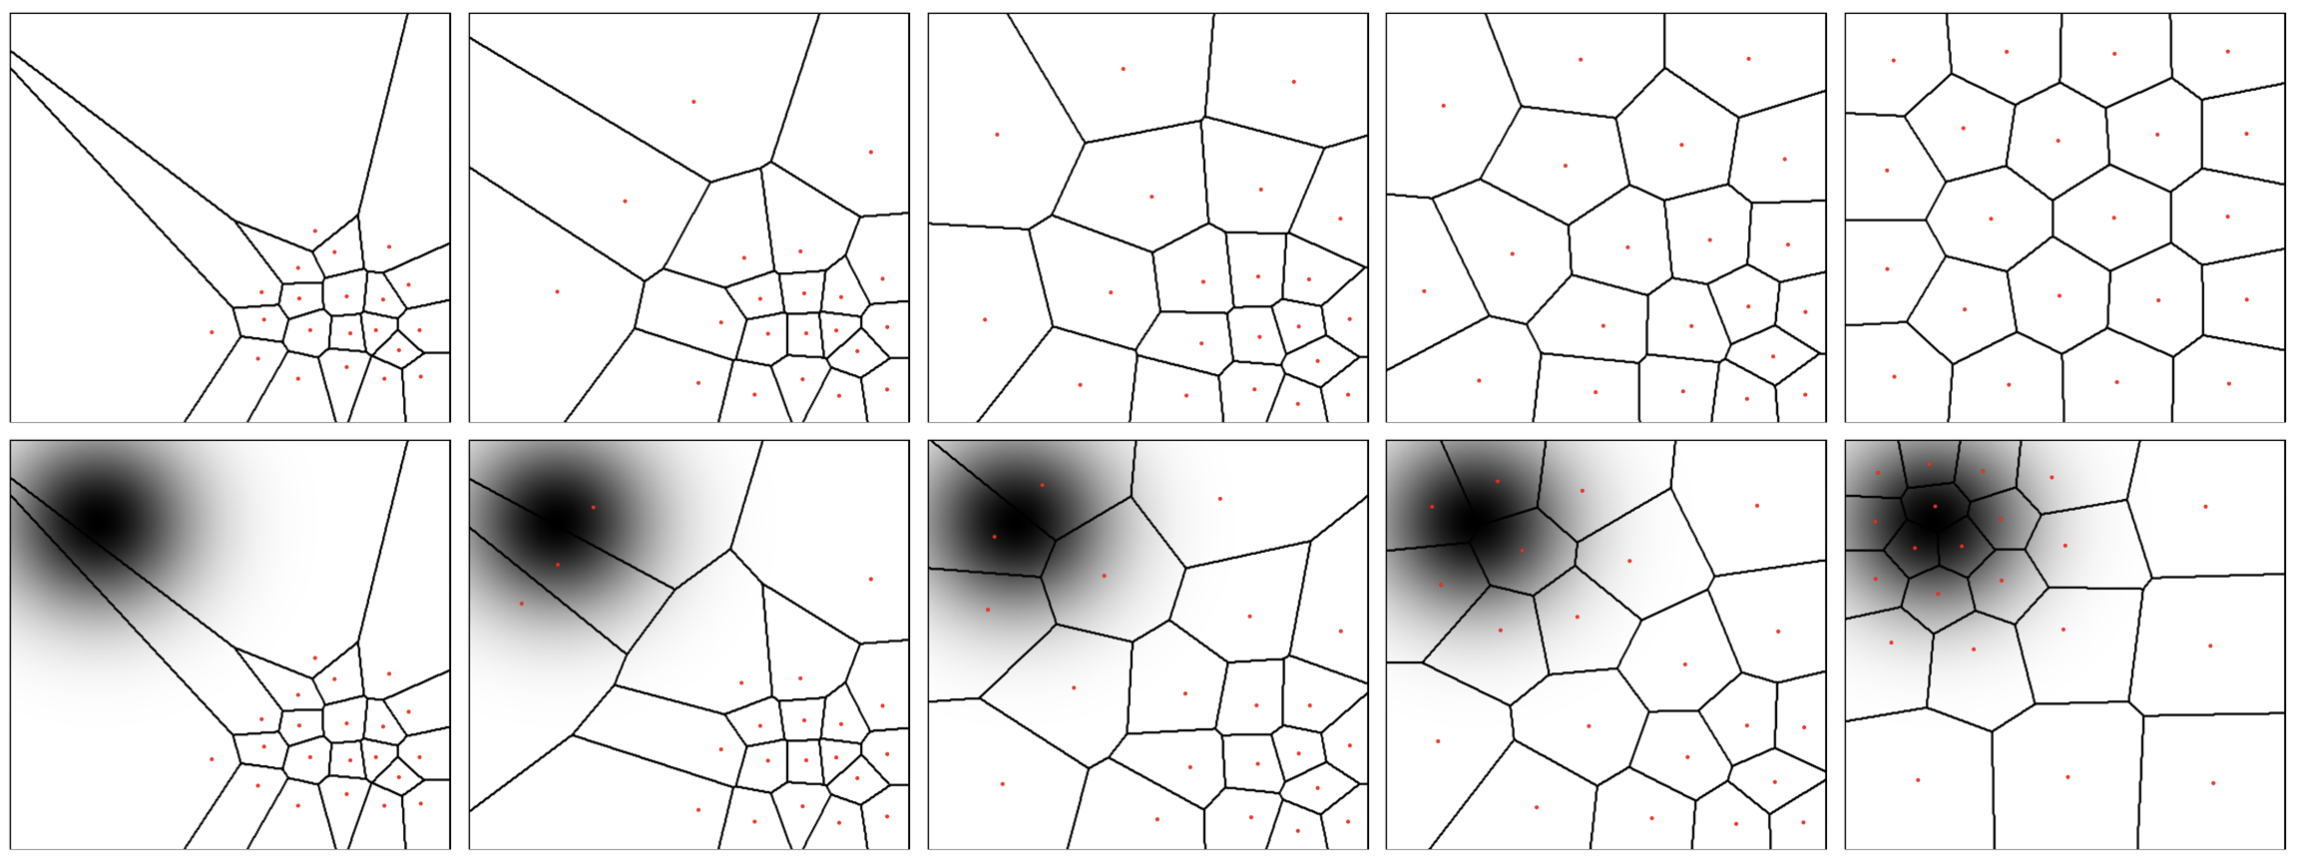
\includegraphics[width=\linewidth]{ml/pca-nn/lloyd}
\caption{\label{fig-lloyd}
Iteration of $k$-means algorithm (Lloyd algorithm) on continuous densities $\mu$. Top: uniform. Bottom: non-uniform (the densities of $\mu$ with respect to the Lebesgue measure is displayed as a grayscale image in the background).
}
\end{figure}




%%%%%%%%%%%%%%%%%%%%%%%%%%%%%%%%%%%%%%%%%%%%%%%%%%
%%%%%%%%%%%%%%%%%%%%%%%%%%%%%%%%%%%%%%%%%%%%%%%%%%
%%%%%%%%%%%%%%%%%%%%%%%%%%%%%%%%%%%%%%%%%%%%%%%%%%
\section{Empirical Risk Minimization}

Before diving into the specifics of regression and classification problems, let us give describe a generic methodology which can be applied in both case (possibly with minor modification for classification, typically considering class probabilities instead of class labels).

In order to make the problem tractable computationally, and also in order to obtain efficient prediction scores, it is important to restrict the fit to the data $y_i \approx f(x_i)$ using a ``small enough'' class of functions. Intuitively, in order to avoid overfitting, the ``size'' of this class of functions should grows with the number $n$ of samples. 

%%%%%%%%%%%%%%%%%%%%%%%%%%%%%%%%%%%%%%%%%%%%%%%%%%
\subsection{Empirical Risk}

Denoting $\Ff_n$ some class of functions (which depends on the number of available samples), one of the most usual way to do the learning is to perform an empirical risk minimization (ERM)
\eql{\label{eq-erm-1}
	\hat f \in \uargmin{f \in \Ff_n} \frac{1}{n} \sum_{i=1}^n \loss(f(x_i),y_i).
}
Here $\loss : \Yy^2 \rightarrow \RR^+$ is the so-called loss function, and it should typically satisfies $\loss(y,y')=0$ if and only if $y=y'$. %
The specifics of $\loss$ depend on the application at hand (in particular, one should use different losses for classification and regression tasks). 
%
To highlight the dependency of $\hat f$ on $n$, we occasionally write $\hat f_n$. 


%%%%%%%%%%%%%%%%%%%%%%%%%%%%%%%%%%%%%%%%%%%%%%%%%%
\subsection{Prediction and Consistency}

When doing a mathematically analysis, one usually assumes that $(x_i,y_i)$ are drawn from a distribution $\pi$ on $\Xx \times \Yy$, and the large $n$ limit defines the ideal estimator
\eql{\label{eq-consistency-estim}
	\bar f \in \uargmin{f \in \Ff_\infty} \int_{\Xx \times \Yy} \loss(f(x),y) \d\pi(x,y) = \EE_{(\xp,\yp) \sim \pi}(\loss(f(\xp),\yp).
}
Intuitively, one should have $\hat f_n \rightarrow \bar f$ as $n \rightarrow +\infty$, which can be captured in expectation of the prediction error over the samples $(x_i,y_i)_i$, i.e.
\eq{
	E_n \eqdef \EE( \tilde\loss(\hat f_n(\xp),\bar f(\xp)) ) \longrightarrow 0.
}
One should be careful that here the expectation is over both $\xp$ (distributed according to the marginal $\pi_\Xx$ of $\pi$ on $\Xx$), and also the $n$ i.i.d. pairs $(x_i,y_i) \sim \pi$ used to define $\hat f_n$ (so a better notation should rather be $(\xp_i,\yp_i)_i$.
%
Here $\bar\loss$ is some loss function on $\Yy$ (one can use $\bar\loss=\loss$ for instance).
One can also study convergence in probability, i.e. 
\eq{
	\foralls \epsilon>0, \quad
	E_{\epsilon,n} \eqdef \PP( \tilde\loss(\hat f_n(\xp),\bar f(\xp)) > \epsilon ) \rightarrow 0.
}
If this holds, then one says that the estimation method is consistent (in expectation or in probability). 
%
The question is then to derive convergence rates, i.e. to upper bound $E_n$ or $E_{\epsilon,n}$ by some explicitly decay rate. 

Note that when $\tilde\loss(y,y')=|y-y'|^r$, then convergence in expectation is stronger (implies) than convergence in probability since using Markov's inequality
\eq{
	E_{\epsilon,n} = \PP( |\hat f_n(\xp)-f(\xp)|^r \geq \epsilon )  \leq \frac{1}{\epsilon} \EE( |\hat f_n(\xp)-f(\xp)|^r ) = \frac{E_n}{\epsilon}.
}

%%%%%%%%%%%%%%%%%%%%%%%%%%%%%%%%%%%%%%%%%%%%%%%%%%
\subsection{Parametric Approaches and Regularization}

Instead of directly defining the class $\Ff_n$ and using it as a constraint, it is possible to rather use a penalization using some prior to favor ``simple'' or ``regular'' functions. 
%
A typical way to achieve this is by using a parametric model $y \approx f(x,\be)$ where $\be \in \Bb$ parametrizes the function $f(\cdot,\be) : \Xx \rightarrow \Yy$. The empirical risk minimization procedure~\eqref{eq-erm-1} now becomes 
\eql{\label{eq-erm-param}
	\hat \be \in \uargmin{\be \in \Bb} \frac{1}{n} \sum_{i=1}^n \loss(f(x_i,\be),y_i) + \la_n J(\be).
}
where $J$ is some regularization function, for instance $J=\norm{\cdot}_2^2$ (to avoid blowing-up of the parameter) or $J=\norm{\cdot}_1$ (to perform model selection, i.e. using only a sparse set of feature among a possibly very large pool of $p$ features). Here $\la_n>0$ is a regularization parameter, and it should tend to $0$ when $n \rightarrow +\infty$. 

Then one similarly defines the ideal parameter $\bar \be$ as in~\eqref{eq-consistency-estim} so that the limiting estimator as $n \rightarrow +\infty$ is of the form $\bar f = f(\cdot,\bar \be)$ for $\bar \be$ defined as
\eql{\label{eq-consistency-param}
	\bar \be \in \uargmin{\be} \int_{\Xx \times \Yy} \loss(f(x,\be),y) \d\pi(x,y) = \EE_{(\xp,\yp) \sim \pi}(\loss(f(\xp,\be),\yp).
}



%%
\paragraph{Prediction vs. estimation risks.}

In this parametric approach, one could be interested in also studying how close $\hat \th$ is to $\bar \th$. This can be measured by controlling how fast some estimation error $\norm{\hat\be-\bar\be}$ (for some norm $\norm{\cdot}$) goes to zero. Note however that in most cases, controlling the estimation error is more difficult than doing the same for the prediction error. In general, doing a good parameter estimation implies doing a good prediction, but the converse is not true. 


%%%%%%%%%%%%%%%%%%%%%%%%%%%%%%%%%%%%%%%%%%%%%%%%%%
\subsection{Testing Set and Cross-validation}

It is not possible to access $E_n$ or $E_{\epsilon,n}$ because the optimal $\bar f$ is unknown. 
%
In order to tune some parameters of the methods (for instance the regularization parameter $\la$), one rather wants to minimize the risk $\EE(L(\hat f(\xp),\yp))$, but this one should not be approximated using the training samples $(x_i,y_i)_i$.

%
One thus rather ressorts to a second set of data $(\bar x_j,\bar y_j)_{j=1}^{\bar n}$, called ``testing set''. From a modelling perspective, this set should also be distributed i.i.d. according to $\pi$. The validation (or testing) risk is then
\eql{\label{eq-valid-risk}
	R_{\bar n} = \frac{1}{\bar n} \sum_{j=1}^{\bar n} \loss(\hat f(\bar x_j),\bar y_j)
}
which converges to $\EE(L(\hat f(\xp),\yp))$ for large $\bar n$.
%
Minimizing $R_{\bar n}$ to setup to some meta-parameter of the method (for instance the regularization parameter $\la_n$) is called ``cross validation'' in the literature.


%%%%%%%%%%%%%%%%%%%%%%%%%%%%%%%%%%%%%%%%%%%%%%%%%%
%%%%%%%%%%%%%%%%%%%%%%%%%%%%%%%%%%%%%%%%%%%%%%%%%%
%%%%%%%%%%%%%%%%%%%%%%%%%%%%%%%%%%%%%%%%%%%%%%%%%%
\section{Supervised Learning: Regression}
\label{sec-regression}

\wrapf{ml/proba-model}{Probabilistic modelling.}
In supervised learning, one has access to training data, consisting in pairs $(x_i,y_i) \in \Xx \times \Yy$. Here $\Xx=\RR^p$ for simplicity. The goal is to infer some relationship, typically of the form $y_i \approx f(x_i)$ for some deterministic function $f : \Xx \rightarrow \Yy$, in order, when some un-observed data $x$ without associated value in $\Yy$ is given, to be able to ``predict'' the associated value using $y = f(x)$. 

If the set $\Yy$ is discrete and finite, then this problem is called a supervised classification problem, and this is studied in Section~\ref{sec-classif}. The simplest example being the binary classification case, where $\Yy=\{0,1\}$. It finds applications for instance in medical diagnosis, where $y_i=0$ indicates a healthy subject, why $y_i=0$ a pathological one.
%
If $\Yy$ is continuous (the typical example being $\Yy=\RR$), then this problem is called a regression problem. 

%%%%%%%%%%%%%%%%%%%%%%%%%%%%%%%%%%%%%%%%%%%%%%%%%%
\subsection{Linear Regression}
\label{sec-linear-models}

We now specialize the empirical risk minimization approach to regression problems, and even more specifically, we consider $\Yy=\RR$ and use a quadratic loss $\loss(y,y')=\frac{1}{2}|y-y'|^2$.

Note that non-linear regression can be achieved using approximation in dictionary (e.g. polynomial interpolation), and this is equivalent to using lifting to a higher dimensional space, and is also equivalent to kernelization technics studied in Section~\ref{sec-kernel-methods}. 

%%%
\paragraph{Least square and conditional expectation.}

If one do not put any constraint on $f$ (beside being measurable), then the optimal limit estimator $\bar f(x)$ defined in~\eqref{eq-consistency-estim} is simply averaging the values $y$ sharing the same $x$, which is the so-called conditional expectation. 
%
Assuming for simplicity that $\pi$ has some density $\frac{\d \pi}{\d x \d y}$ with respect to a tensor product measure $\d x \d y$ (for instance the Lebegues mesure), one has
\eq{
	\foralls x \in \Xx, \quad
	\bar f(x) = \EE( \yp | \xp=x) = 
	\frac{ 
		\int_{\Yy} y \frac{\d \pi}{\d x \d y}(x,y) \d y 
	}{ 
		\int_{\Yy} \frac{\d \pi}{\d x \d y}(x,y) \d y
	 }
}
where $(\xp,\yp)$ are distributed according to $\pi$.


\begin{figure}
\centering
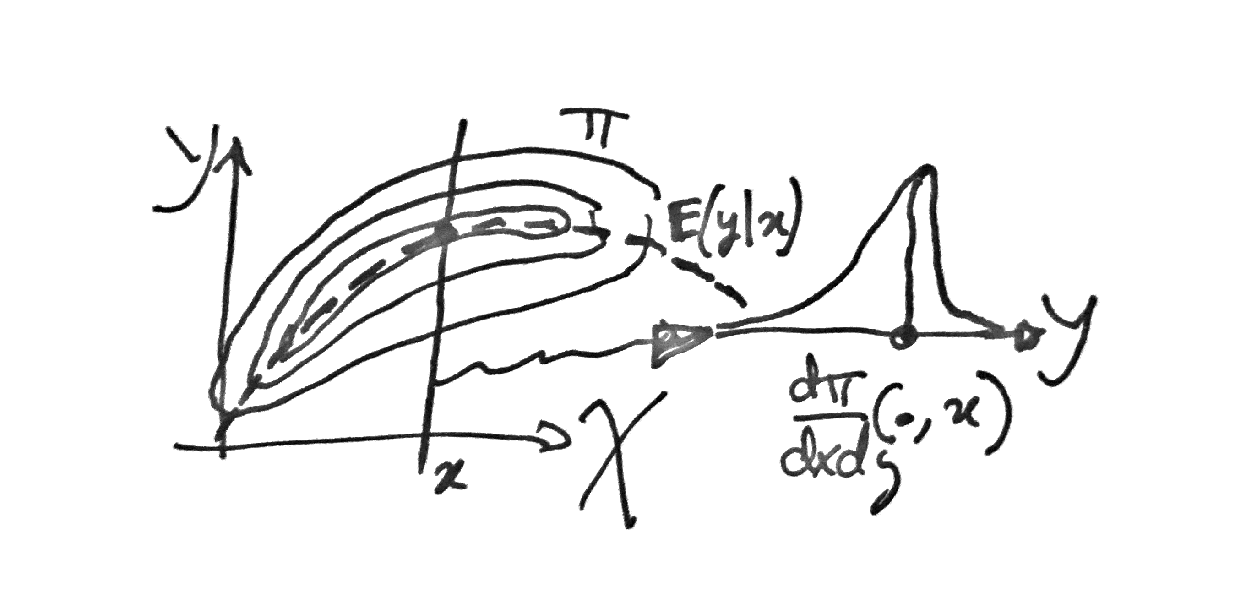
\includegraphics[width=.5\linewidth]{ml/cond-expect}
\caption{\label{fig-bound-regul}
Conditional expectation.
}
\end{figure}

In the simple case where $\Xx$ and $\Yy$ are discrete, denoting $\pi_{x,y}$ the probability of $(\xp=x,\yp=y)$, one has
\eq{
	\foralls x \in \Xx, \quad
	\bar f(x) = \frac{ \sum_{y}  y \pi_{x,y} }{ \sum_{y} \pi_{x,y} }
}
and it is unspecified if the marginal of $\pi$ along $\Xx$ vanishes at $x$. 

The main issue is that this estimator $\hat f$ performs poorly on finite samples, and $f(x)$ is actually undefined if there is no sample $x_i$ equal to $x$. This is due to the fact that the class of functions is too large, and one should impose some regularity or simplicity on the set of admissible $f$.


%%%
\paragraph{Penalized linear models.}

\wrapf{ml/linear-fit}{Linear regression.}
A very simple class of models is obtained by imposing that $f$ is linear, and set $f(x,\be)=\dotp{x}{\be}$, for parameters $\be \in \Bb=\RR^p$. Note that one can also treat this way affine functions by remarking that $\dotp{x}{\be}+\be_0=\dotp{(x,1)}{(\be,\be_0)}$ and replacing $x$ by $(x,1)$.  So in the following, without loss of generality, we only treat the vectorial (non-affine) case. 

Under the square loss, the regularized ERM~\eqref{eq-erm-param} is conveniently rewritten as 
\eql{\label{eq-erm-lin}
	\hat \be \in \uargmin{\be \in \Bb} \frac{1}{2} \dotp{\hat C \be}{\be} - \dotp{\hat u}{\be} + \la_n J(\be)
}
where we introduced the empirical correlation (already introduced in~\eqref{eq-emp-cov}) and observations
\eq{
	\hat C \eqdef \frac{1}{n} X^* X = \frac{1}{n} \sum_{i=1}^n x_i x_i^*
	\qandq
	\hat u \eqdef \frac{1}{n} \sum_{i=1}^n y_i x_i = \frac{1}{n} X^* y \in \RR^p.
}
As $n \rightarrow 0$, under weak condition on $\pi$, one has with the law of large numbers the almost sure convergence
\eql{\label{eq-empirical-conver}
	\hat C \rightarrow C \eqdef \EE(\xp^* \xp)
	\qandq
	\hat u \rightarrow u \eqdef \EE(\yp \xp).
}
When considering $\la_n \rightarrow 0$, in some cases, one can shows that in the limit $n \rightarrow +\infty$, one retrieves the following ideal parameter 
\eq{
	\bar \be \in \uargmin{\be} \enscond{ J(\be) }{ C\be=u }.
}

Problem~\eqref{eq-erm-lin} is equivalent to the regularized resolution of inverse problems~\eqref{eq-regul-inv}, with $\hat C$ in place of $\Phi$ and $\hat u$ in place of $\Phi^* y$.
%
The major, and in fact only difference between machine learning and inverse problems is that the linear operator is also noisy since $\hat C$ can be viewed as a noisy version of $C$. The ``noise level'', in this setting, is $1/\sqrt{n}$ in the sense that
\eq{
	\EE(\norm{\hat C-C}) \sim \frac{1}{\sqrt{n}}
	\qandq
	\EE(\norm{\hat u-u}) \sim \frac{1}{\sqrt{n}}, 
}
under the assumption that $\EE(\yp^4)<+\infty$, $\EE(\norm{\xp}^4)<+\infty$ so ensure that one can use the central limit theorem on $\xp^2$ and $\xp\yp$. Note that, although we use here linear estimator, one does not need to assume a ``linear'' relation of the form $\yp=\dotp{\xp}{\be} + w$ with a noise $w$ independent from $\xp$, but rather hope to do ``as best as possible'', i.e. estimate a linear model as close as possible to $\bar\be$. 

The general take home message is that it is possible to generalize Theorems~\ref{thm-sublin-quad}, \ref{thm-bregman-rates} and~\ref{thm-linrate-l1} to cope with the noise on the covariance matrix to obtain prediction convergence rates of the form 
\eq{
	\EE( |\dotp{\hat \be}{\xp}-\dotp{\bar \be}{\xp}|^2 ) = O( n^{-\kappa} )
}
and estimation rates of the form 
\eq{
	\EE( \norm{\hat \be-\bar \be}^2  ) = O( n^{-\kappa'} ), 
}
under some suitable source condition involving $C$ and $u$.
%
Since the noise level is roughly $n^{-\frac{1}{2}}$, the ideal cases are when $\kappa=\kappa'=1$, which is the so-called linear rate regime.  
%
It is also possible to derive sparsistency theorems by extending theorem~\ref{thm-support-stable}. For the sake of simplicity, we now focus our attention to quadratic penalization, which is by far the most popular regression technic. It is fair to say that sparse (e.g. $\ell^1$ type) methods are not routinely used in machine learning, because they typically do not improve the estimation performances, and are mostly useful to do model selection (isolate a few useful coordinates in the features). 
%
This is in sharp contrast with the situation for inverse problems in imaging sciences, where sparsity is a key feature because it corresponds to a modelling assumption on the structure of the data to recover. 

%%%
\paragraph{Ridge regression (quadratic penalization).}

For $J=\norm{\cdot}^2/2$, the estimator~\eqref{eq-erm-lin} is obtained in closed form as
\eql{\label{eq-linest-std}
	\hat\be = ( X^* X + n\la_n \Id_p )^{-1} X^* y = 
	( \hat C + n \la_n \Id )^{-1} \hat u. 
}
This is often called ridge regression in the literature.
%
Note that thanks to the Woodbury formula, this estimator can also be re-written as
\eql{\label{eq-linest-woodbury}
	\hat\be = X^* ( XX^* + n\la_n \Id_n )^{-1}  y .
}
If $n \gg p$ (which is the usual setup in machine learning), then~\eqref{eq-linest-woodbury} is preferable. In some cases however (in particular when using RKHS technics), it makes sense to consider very large $p$ (even infinite dimensional), so that~\eqref{eq-linest-std} must be used. 

If $\la_n \rightarrow 0$, then using~\eqref{eq-empirical-conver}, one has the convergence in expectation and probability
\eq{
	\hat\be \rightarrow \bar\be = C^{+} u. 
}
Theorems~\ref{thm-sublin-quad} and~\ref{thm-bregman-rates} can be extended to this setting and one obtains the following result.

\begin{thm}
	If
	\eql{\label{eq-sc-stat}
		\bar\be = C^{\gamma} z
		\qwhereq 
		\norm{z} \leq \rho
	}
	for $0 < \gamma \leq 2$, then 
	\eql{\label{eq-rate-estim}
		\EE( \norm{\hat \be-\bar \be}^2  ) \leq C \rho^{2 \frac{1}{\ga+1}} n^{-\frac{\ga}{\ga+1}}
	}
	for a constant $C$ depending only on $\ga$.
\end{thm}

It is important to note that, since $\bar\be = C^{+} u$, the source condition~\eqref{eq-sc-stat} is always satisfied. What trully matters here is that the rate~\eqref{eq-rate-estim} does not depend on the dimension $p$ of the features, but rather only on $\rho$, which can be much smaller. This theoretical analysis actually works perfectly fine in infinite dimension $p=\infty$ (which is the setup considered when dealing with RKHS bellow). 


%%%%%%%%%%%%%%%%%%%%%%%%%%%%%%%%%%%%%%%%%%%%%%%%%%
%%%%%%%%%%%%%%%%%%%%%%%%%%%%%%%%%%%%%%%%%%%%%%%%%%
%%%%%%%%%%%%%%%%%%%%%%%%%%%%%%%%%%%%%%%%%%%%%%%%%%
\section{Supervised Learning: Classification}
\label{sec-classif}

We now focus on the case of discrete labels $y_i \in \Yy = \{1,\ldots,k\}$, which is the classification setup.
%
We now detail two popular classification methods: nearest neighbors and logistic classification.
%
It is faire to say that a significant part of successful applications of machine learning technics consists in using one of these two approaches, which should be considered as baselines. 
%
Note that the nearest neighbors approach, while popular for classification could as well be used for regression.

%%%%%%%%%%%%%%%%%%%%%%%%%%%%%%%%%%%%%%%%%%%%%%%%%%%%%%%%%%%%%%%%%%%%%%%%%%%%%%%%%%%%%%%%%%%%%%%%%%%%%%%%%%%%
\subsection{Nearest Neighbors Classification}
\label{sec-nn-classif}

Probably the simplest method for supervised classification is $R$ nearest neighbors ($R$-NN), where $R$ is a parameter indexing the number of neighbors. Increasing $R$ is important to cope with noise and obtain smoother decision boundaries, and hence better generalization performances. It should typically decreases as the number of training samples $n$ increases.
%
Despite its simplicity, $k$-NN is surprisingly successful in practice, specially in low dimension $p$.

The class $\hat f(x) \in \Yy$ predicted for a point $x$ is the one which is the most represented among the $R$ points $(x_i)_i$ which are the closed to $x$. This is a non-parametric method, and $\hat f$ depends on the numbers $n$ of samples (its ``complexity'' increases with $n$). 

\wrapf{ml/clustering}{Nearest neighbors.}
One first compute the Euclidean distance between this $x$ 
and all other $x_{i}$ in the training set. 
%
Sorting the distances generates an indexing $\si$ (a permutation of $\{1,\ldots,n\}$) such that 
\eq{
 	\norm{x-x_{\si(1)}} \leq \norm{x-x_{\si(2)}} \leq \ldots \leq \norm{x-x_{\si(n)}}. 
}
For a given $R$, one can compute the ``local'' histogram of classes around $x$
\eq{
 	h_\ell(x) \eqdef \frac{1}{R} \enscond{ i }{ y_{\si(i)} \in \{1,\ldots,R\} }.
}
The decision class for $x$ is then a maximum of the histogram
\eq{
	\hat f(x) \in \uargmax{\ell} h_\ell(x).
}

In practice, the parameter $R$ can be setup through cross-validation, by minimizing the testing risk $R_{\bar n}$ defined in~\eqref{eq-valid-risk}, which typically uses a 0-1 loss for counting the number of mis-classifications
\eq{
	R_{\bar n} \eqdef \sum_{j=1}^{\bar n} \de( \bar y_j - \hat f(x_i) )
}
where $\de(0)=0$ and $\de(s)=1$ if $s \neq 0$. 
%
Of course the method extends to arbitrary metric space in place of Euclidean space $\RR^p$ for the features.
%
Note also that instead of explicitly sorting all the Euclidean distance, one can use fast nearest neighbor search methods.
	
\begin{figure}
\centering
\begin{tabular}{@{}c@{\hspace{3mm}}c@{\hspace{3mm}}c@{\hspace{3mm}}c@{\hspace{3mm}}c@{}}
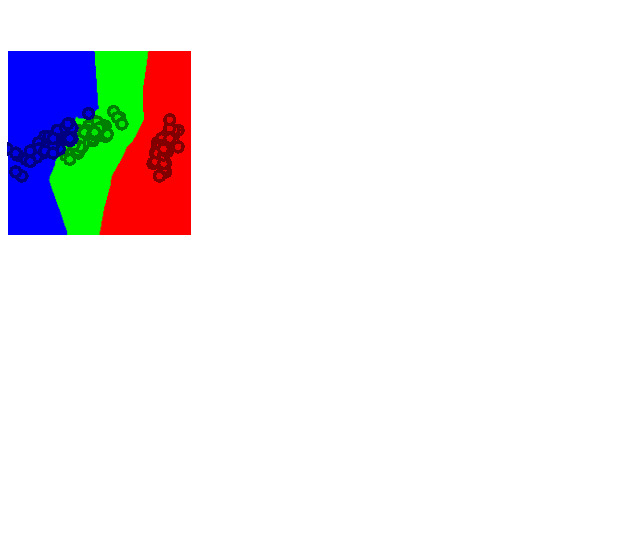
\includegraphics[width=.22\linewidth]{ml/pca-nn/knn-1}&
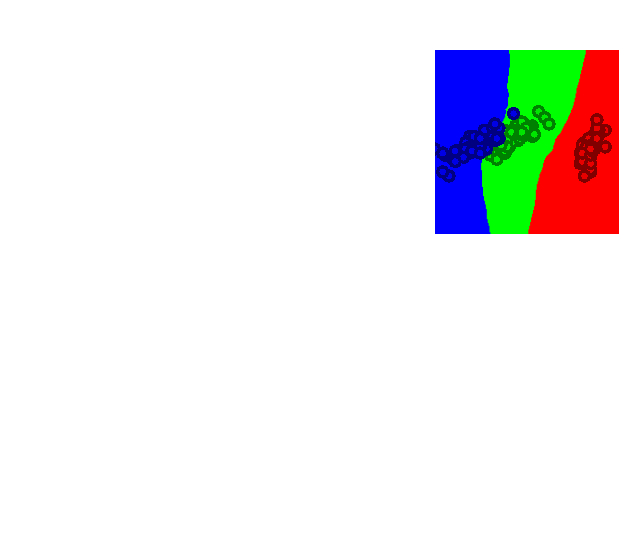
\includegraphics[width=.22\linewidth]{ml/pca-nn/knn-5}&
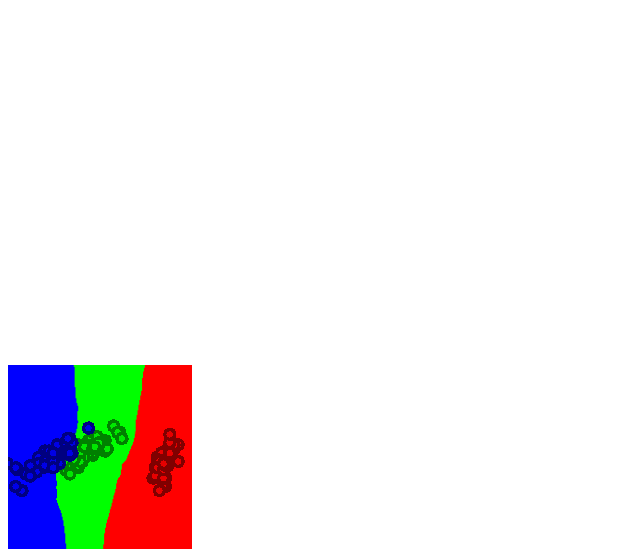
\includegraphics[width=.22\linewidth]{ml/pca-nn/knn-10}&
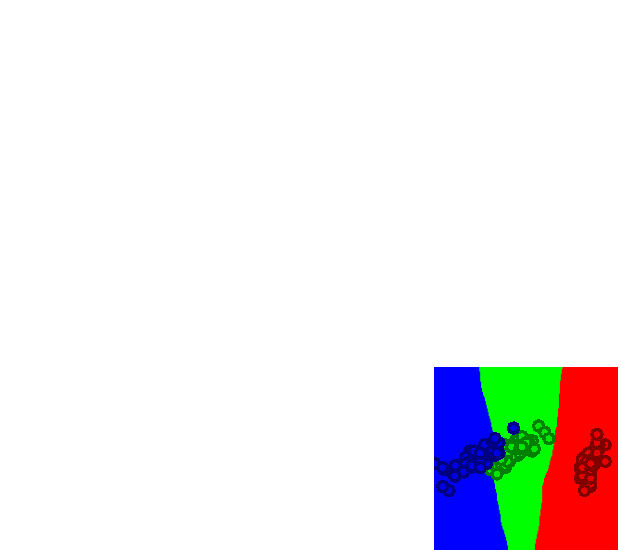
\includegraphics[width=.22\linewidth]{ml/pca-nn/knn-40}\\
$k=1$ & $k=5$ & $k=10$ & $k=40$
\end{tabular}
\caption{\label{fig-hist-classif}
$k$-nearest-neighbor classification boundary function.
}
\end{figure}

Figure~\ref{fig-hist-classif} shows, for the IRIS dataset, the classification domains (i.e. $\enscond{x}{f(x)=\ell}$ for $\ell=1,\ldots,k$)  using a 2-D projection for vizualization.
%
Increasing $R$ leads to smoother class boundaries.

%%%%%%%%%%%%%%%%%%%%%%%%%%%%%%%%%%%%%%%%%%%%%%%%%%
\subsection{Two Classes Logistic Classification}
\label{sec-two-class-logit}

The logistic classification method (for 2 classes and multi-classes) is one of the most popular (maybe ``the'' most) popular machine learning technics. This is due in large part of both its simplicity and because it also outputs a probability of belonging to each class (in place of just a class membership), which is useful to (somehow \ldots) quantify the ``uncertainty'' of the estimation.
%
Note that logistic classification is actually called ``logistic
regression'' in the literature, but it is in fact a classification method.

Another very popular (and very similar) approach is support vector machine (SVM). SVM is both more difficult to train (because the loss is non-smooth) and does not give class membership probability, so the general rule of thumb is that logistic classification is preferable.

To simplify the expression, classes indexes are set to $y_i \in \Yy = \{-1,1\}$ in the following. Note that for logistic classification, the prediction function $f(\cdot,\be) \in [0,1]$ outputs the probability of belonging to the first class, and not the class indexes. With a slight abuse of notation, we still denote it as $f$. 


%%%%
\paragraph{Approximate risk minimization.}

The hard classifier is defines from a linear predictor $\dotp{x}{\be}$ as $\sign(\dotp{x}{\be}) \in \{-1,+1\}$. The 0-1 loss error function (somehow the ``ideal'' loss) counts the number of miss-classifications, and can ideal classifier be computed as
\eql{\label{eq-ideal-classif}
	\umin{\be} \sum_{i=1}^n \ell_0(-y_i \dotp{x_i}{\be})
} 
where $\ell_0 = 1_{\RR^+}$. Indeed, miss classification corresponds to $\dotp{x_i}{w}$ and $y_i$ having different signs, so that in this case $\ell_0(-y_i \dotp{x_i}{w})=1$ (and 0 otherwise for correct classification).

The function $\ell_0$ is non-convex and hence problem~\eqref{eq-ideal-classif} is itself non-convex, and in full generality, can be shown to be NP-hard to solve. One thus relies on some proxy, which are functions which upper-bounds $\ell_0$ and are convex (and sometimes differentiable). 

The most celebrated proxy are 
\eq{
	\ell(u)=(1+u)_+ 
	\qandq
	\ell(u)=\log(1+\exp(u))/\log(2)
}	
which are respectively the hinge loss corresponds to support vector machine (SVM, and is non-smooth) and the logistic loss (which is smooth). The $1/\log(2)$ is just a constant which makes $\ell_0 \leq \ell$.
% 
AdaBoost is using $\ell(u)=e^u$.
%
Note that least square corresponds to using $\ell(u)=(1+u)^2$, but this is a poor proxy for $\ell_0$ for negative values, although it might works well in practice.
% 
Note that SVM is a non-smooth problem, which can be cast as a linear program minimizing the co-called classification margin 
\eq{
	\umin{u \geq 0, \be} \enscond{\sum_i u_i}{1+u_i=y_i \dotp{x_i}{\be} }.
}	


%%%%
\paragraph{Logistic loss probabilistic interpretation.}

Logistic classification can be understood as a linear model as introduced in Section~\ref{sec-linear-models}, although the decision function $f(\cdot,\be)$ is not linear. Indeed, one needs to ``remap'' the linear value $\dotp{x}{\be}$ in the interval $[0,1]$. In logistic classification, we define the predicted probability of $x$ belonging to class with label $-1$ as 
\eql{\label{eq-two-class-logit-model}
	f(x,\be) \eqdef \th(\dotp{x}{\be})
	\qwhereq
   	\th(s) \eqdef \frac{e^{s}}{1+e^s} = (1+e^{-s})^{-1},
}
which is often called the ``logit'' model.
%
Using a linear decision model might seems overly simplistic, but in high dimension $p$, the number of degrees of freedom is actually enough to reach surprisingly good classification performances.
%
Note that the probability of belonging to the second class is $1-f(x,\be)=\th(-s)$. This symmetry of the $\th$ function is important because it means that both classes are treated equally, which makes sense for ``balanced'' problem (where the total mass of each class are roughly equal).

Intuitively, $\be/\norm{\be}$ controls the separating hyperplane direction, while $1/\norm{\be}$ is roughly the fuzziness of the the separation. As $\norm{\be} \rightarrow +\infty$, one obtains sharp devision boundary, and logistic classification ressembles SVM.

\begin{figure}
\centering
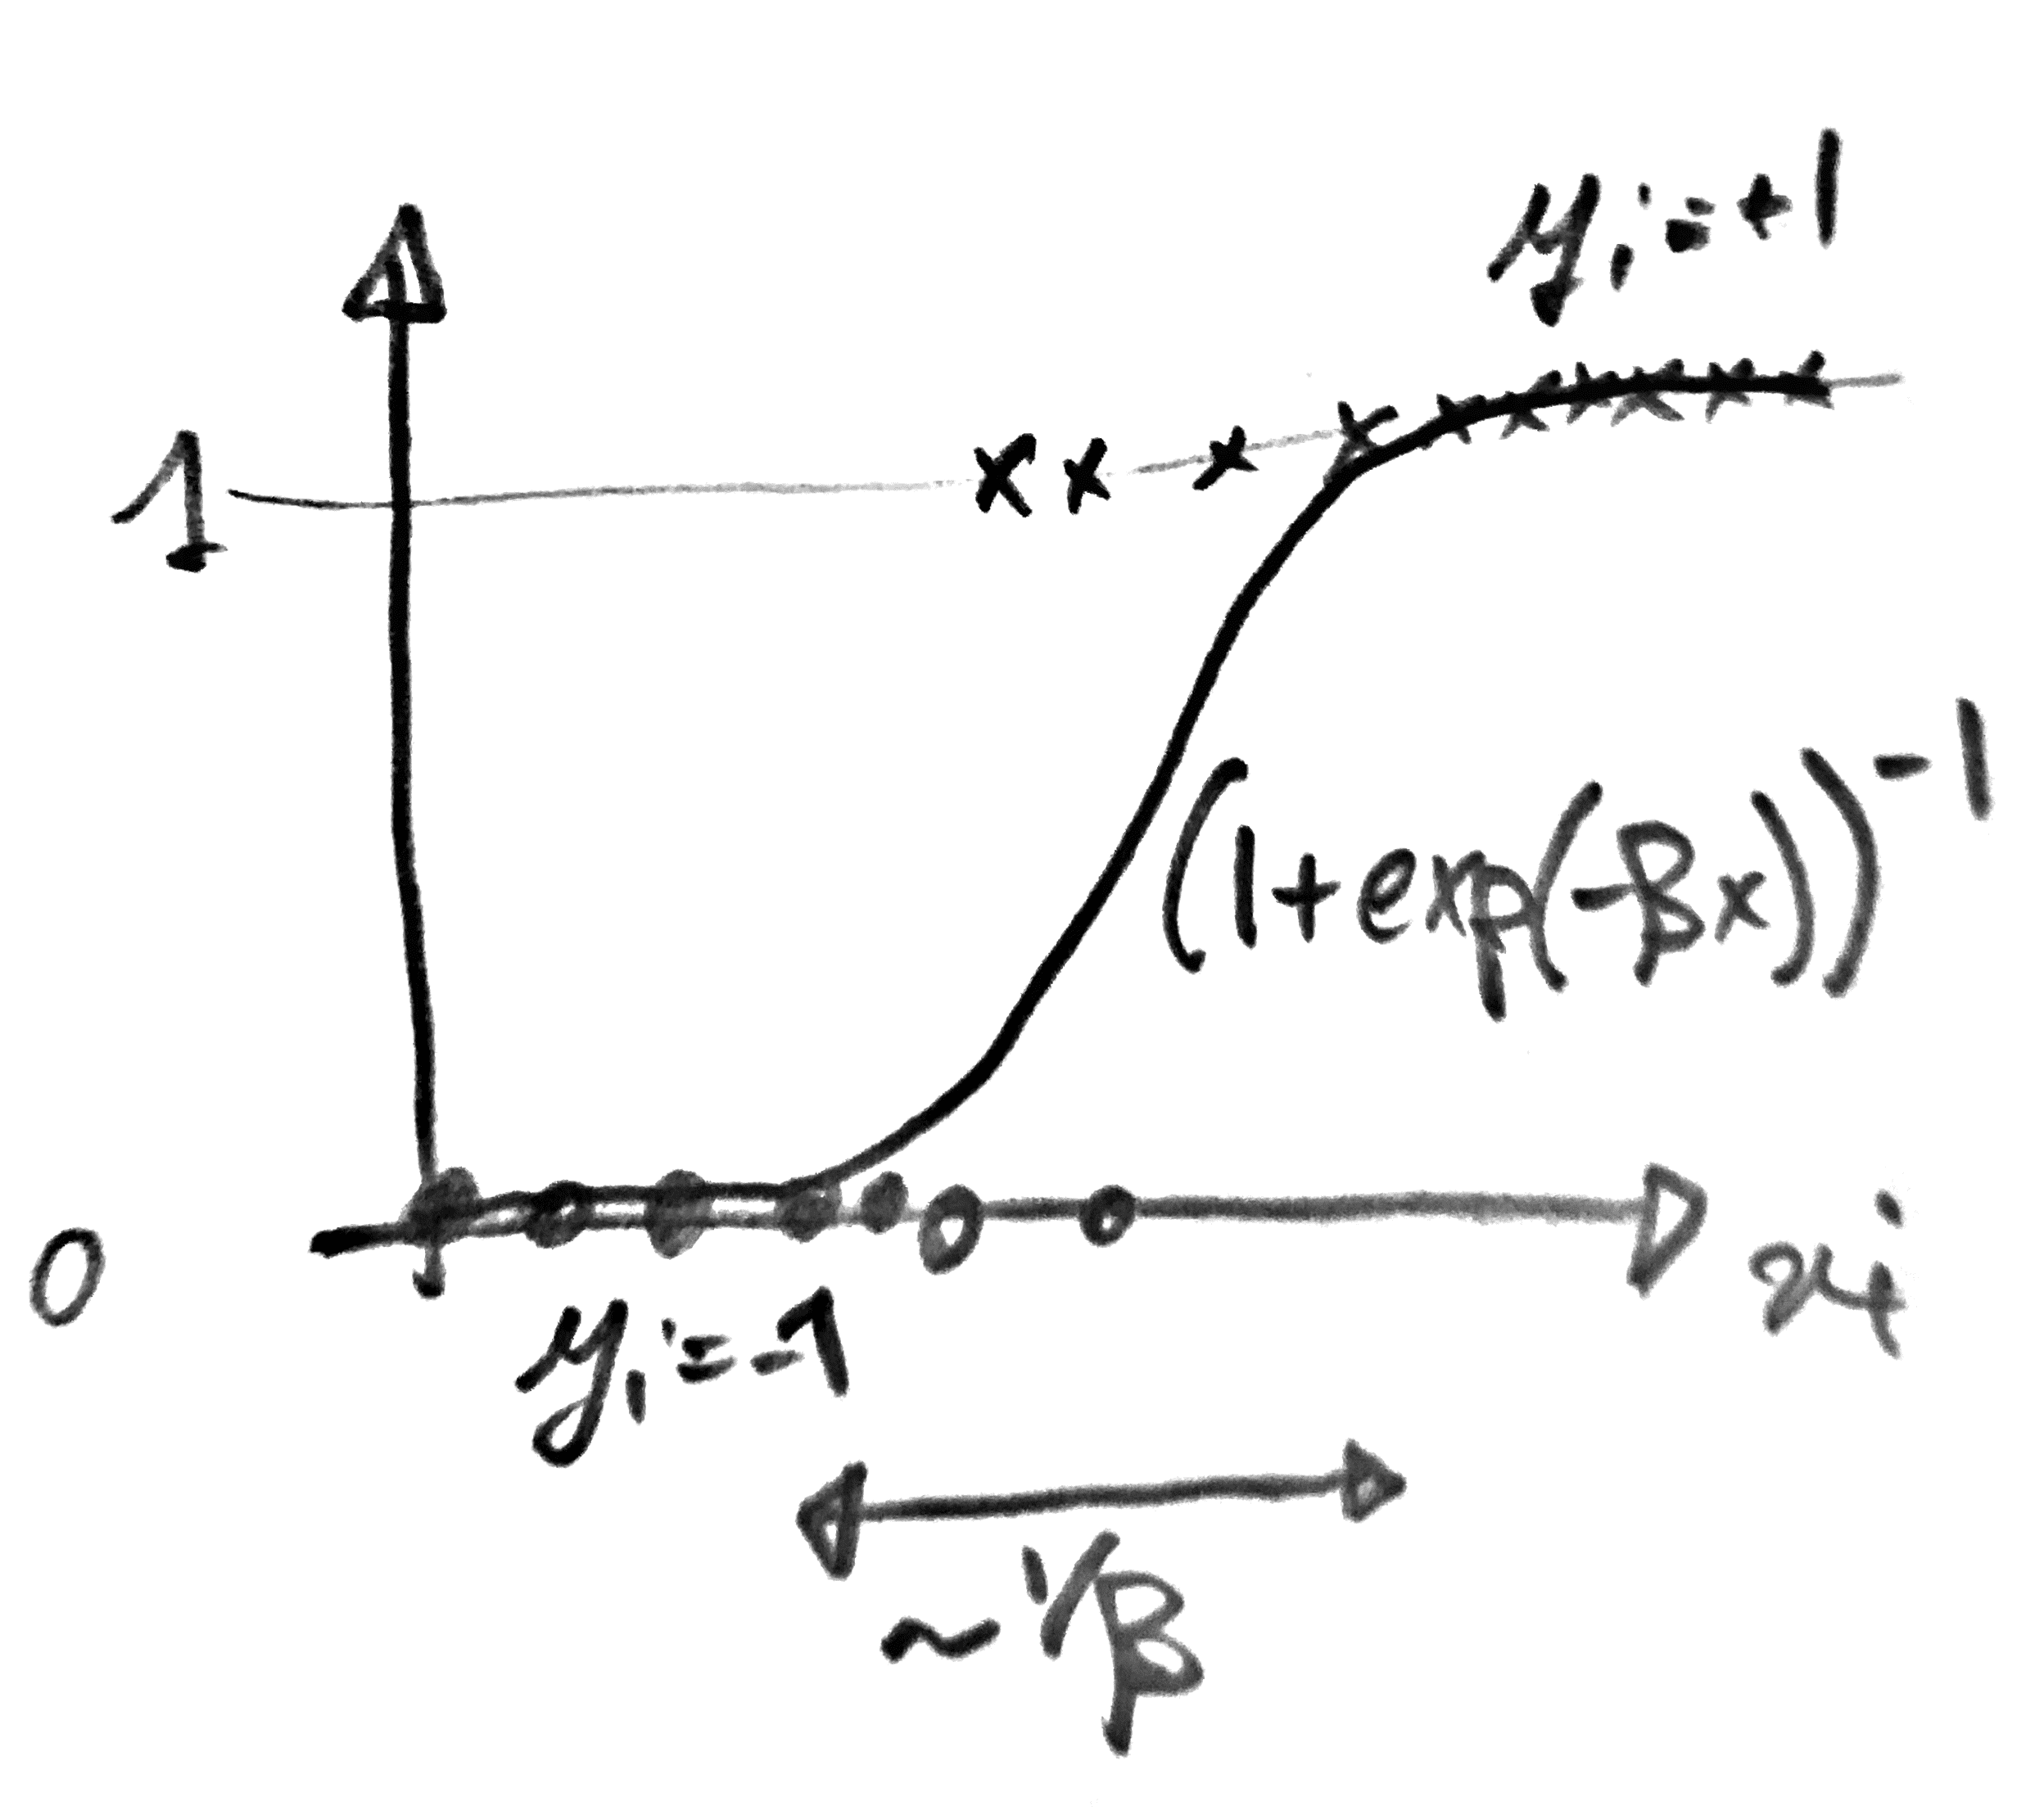
\includegraphics[width=.3\linewidth]{ml/logistic-1d}\qquad
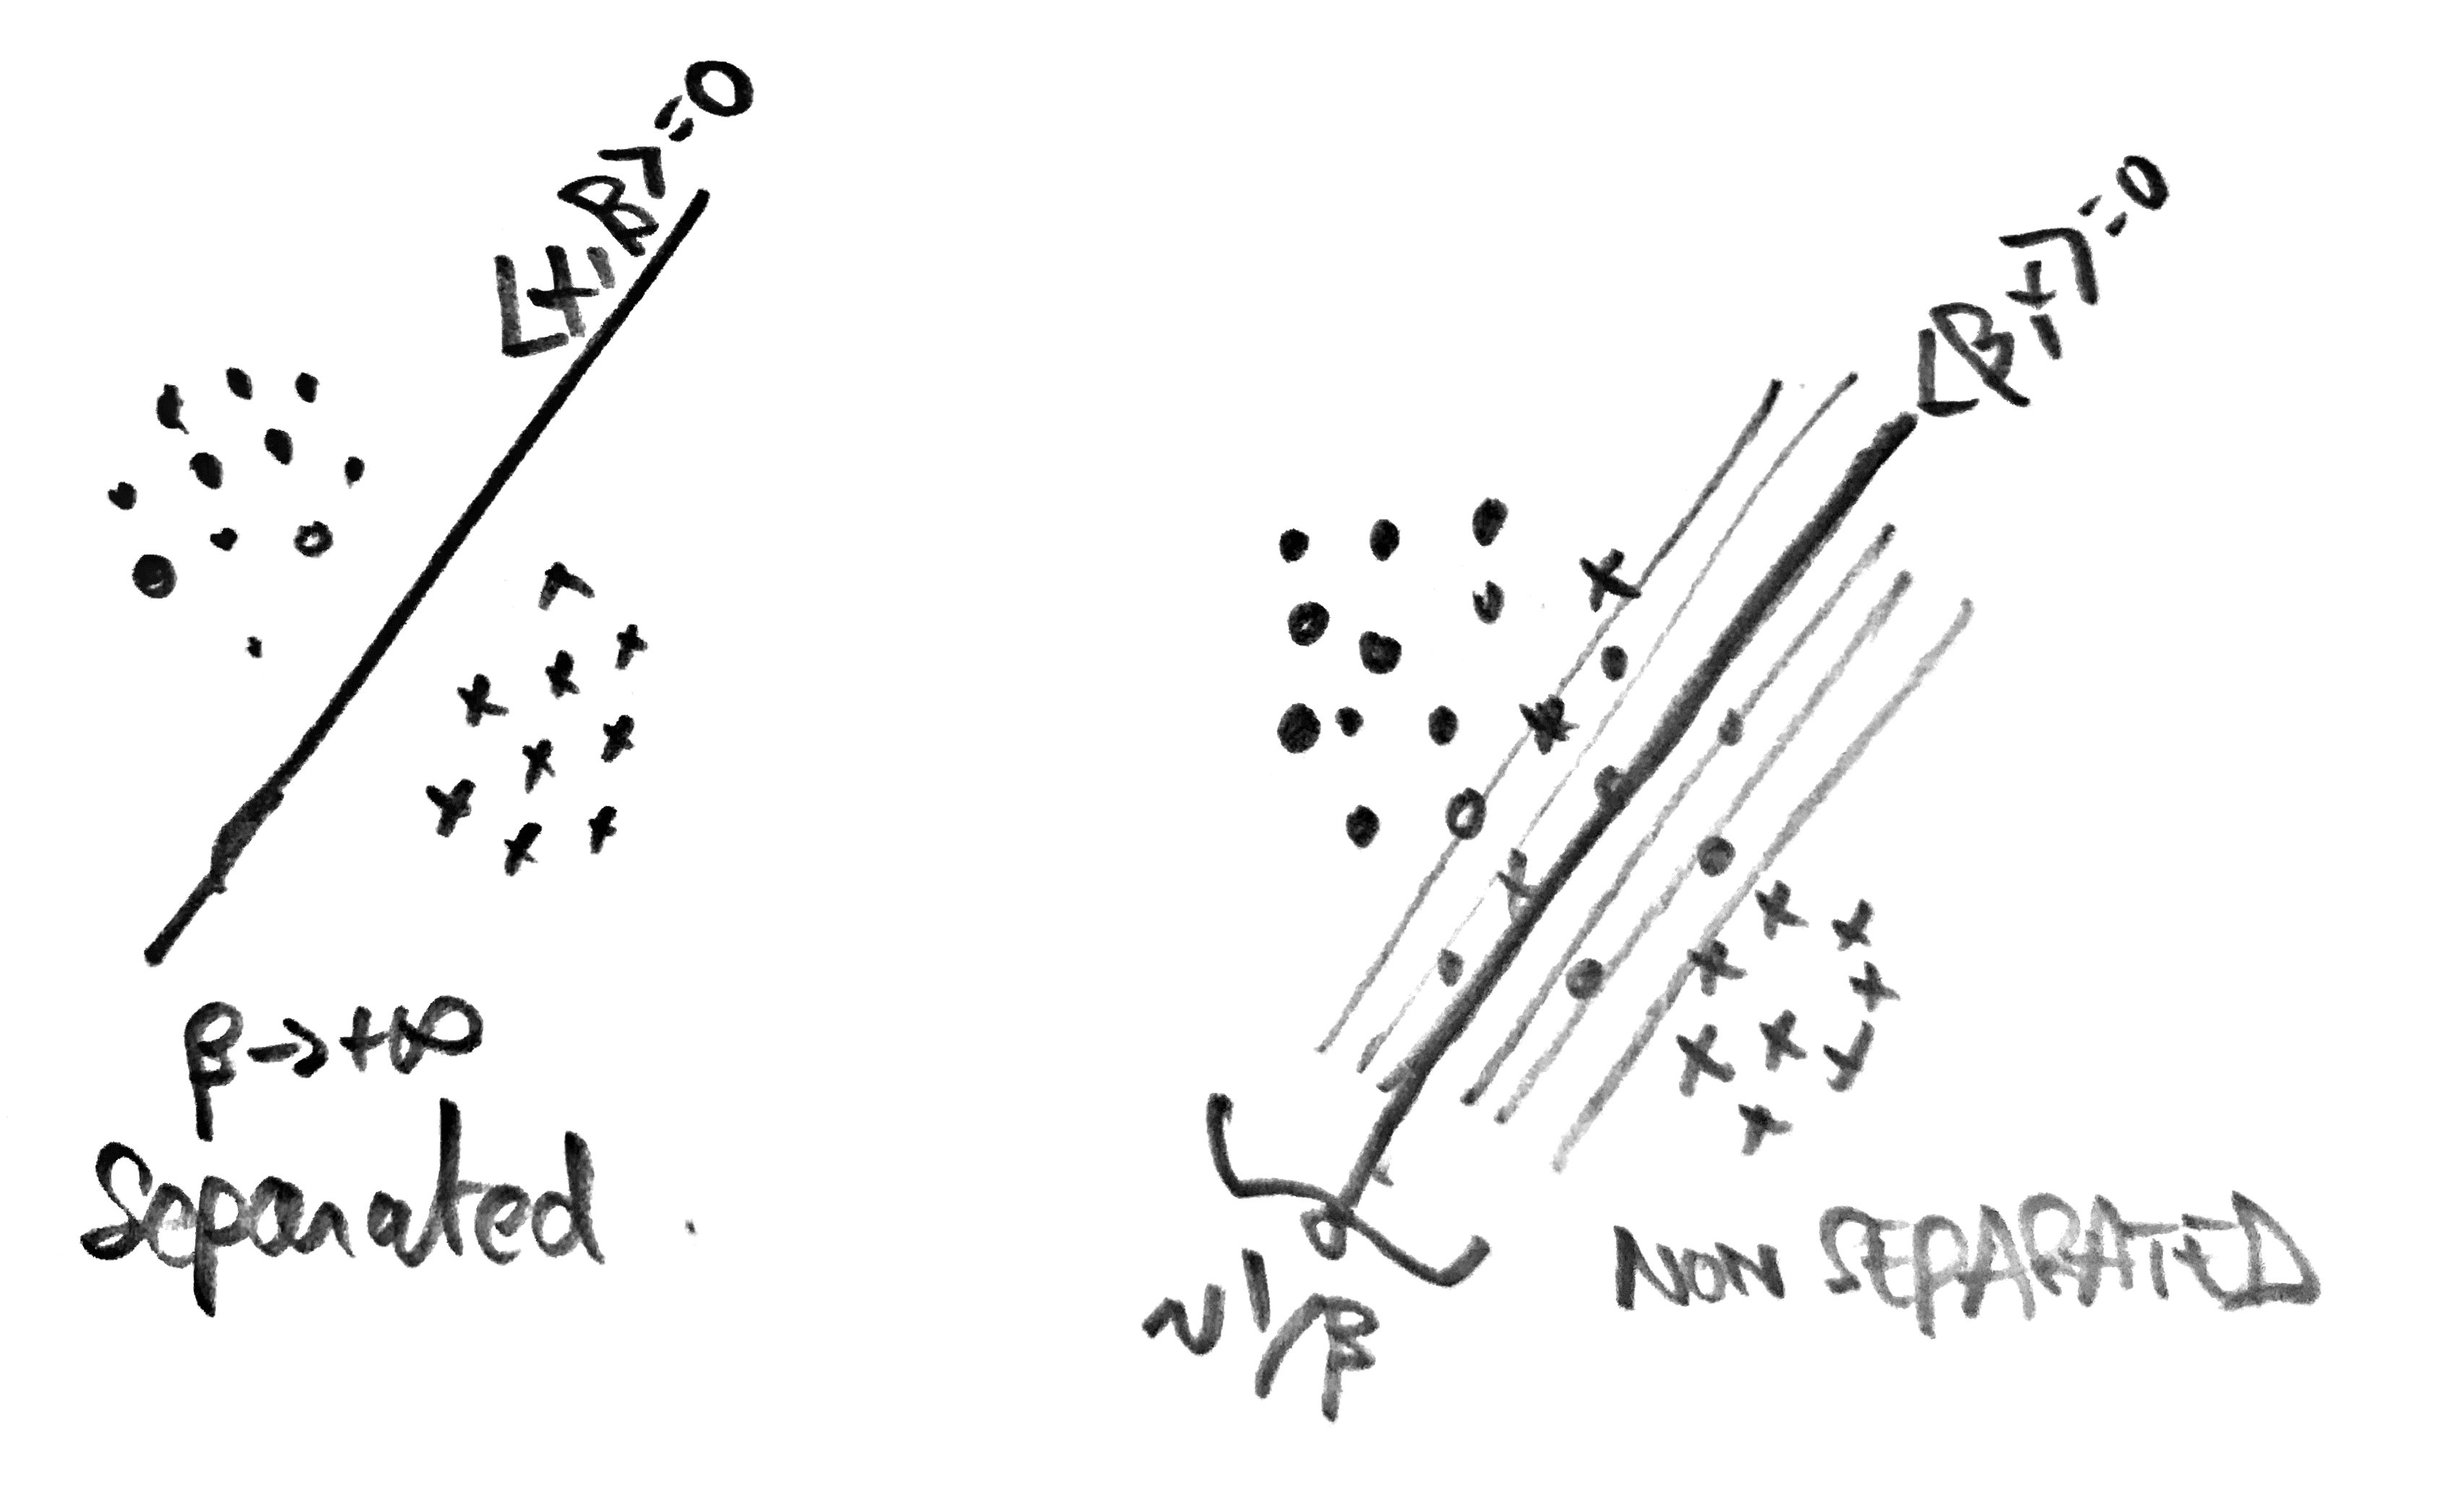
\includegraphics[width=.5\linewidth]{ml/logistic-2d}
\caption{\label{fig-losses}
1-D and 2-D logistic classification, showing the impact of $\norm{\be}$ on the sharpness of the classification boundary.
}
\end{figure}

Note that $f(x,\be)$ can be interpreted as a single layer perceptron with a logistic (sigmoid) rectifying unit, more details on this in Chapter~\ref{c-deep-learning}. 

Since the $(x_i,y_i)$ are modeled as i.i.d. variables, it makes sense to define $\hat \be$ from the observation using a maximum likelihood, assuming that each $y_i$ conditioned on $x_i$ is a Bernoulli variable with associated probability $(p_i,1-p_i)$ with $p_i=f(x_i,\be)$. The probability of observing $y_i \in \{0,1\}$ is thus, denoting $s_i=\dotp{x_i}{\be}$
\eq{
	\PP(\yp=y_i|\xp=x_i) =p_i^{1-\bar y_i} (1-p_i)^{\bar y_i}
	= \pa{
		\frac{e^{s_i}}{1+e^{s_i}}
	}^{1-\bar y_i} 
	\pa{
		\frac{1}{1+e^{s_i}}
	}^{\bar y_i}
}
where we denoted $\bar y_i = \frac{y_i+1}{2} \in \{0,1\}$.

One can then minimize minus the sum of the log of the likelihoods, which reads
\eq{
	\hat\be \in \uargmin{\be \in \RR^p} 
		- \sum_{i=1}^n \log( \PP(\yp=y_i|\xp=x_i) ) = 
		\sum_{i=1}^n - (1-\bar y_i) \log \frac{e^{s_i}}{1+e^{s_i}}
			- \bar y_i\log \frac{1}{1+e^{s_i}}
}
Some algebraic manipulations shows that this is equivalent to an ERM-type form~\eqref{eq-erm-param} with a logistic loss function 
\eql{\label{eq-logistic-optim}
	\hat\be \in \uargmin{\be \in \RR^p} 
		 E(\be)  = \frac{1}{n} \sum_{i=1}^n \loss(\dotp{x_i}{\be},y_i)  
}
where the logistic loss reads
\eql{\label{eq-logistic-loss}
	 \loss( s,y ) \eqdef \log( 1+\exp(-sy) ). 
}
Problem~\eqref{eq-logistic-optim} is a smooth convex minimization. If $X$ is injective, $E$ is also strictly convex, hence it has a single global minimum.

\begin{figure}
\centering
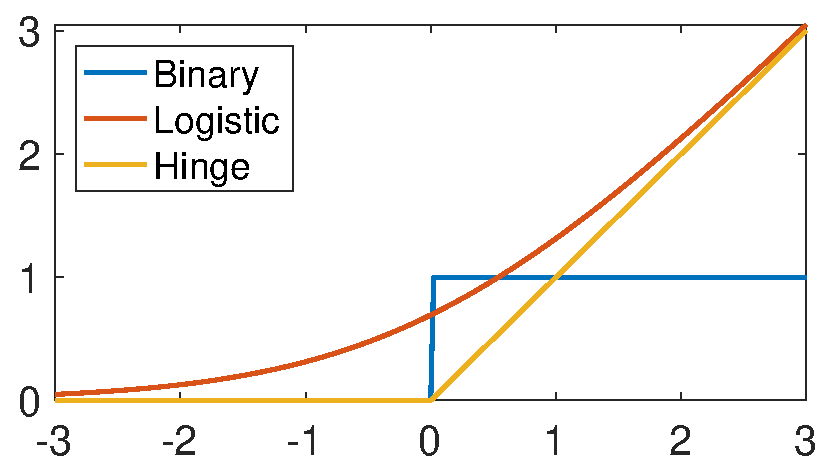
\includegraphics[width=.4\linewidth]{ml/classif/losses}
\caption{\label{fig-losses}
Comparison of loss functions.  \todo{Re-do the figure, it is not correct, they should upper bound $\ell_0$}
}
\end{figure}

Figure~\eqref{fig-losses} compares the binary (ideal) 0-1 loss, the logistic loss and the hinge loss (the one used for SVM).

%%%
\paragraph{Gradient descent method.}

Re-writing the energy to minimize
\eq{
	 E(\be) = \Loss(X \be,y) \qwhereq \Loss(s,y)= \frac{1}{n}  \sum_i \loss(s_i,y_i), 
}
its gradient reads
\eq{
	 \nabla E(\be) = X^* \nabla \Loss(X \be,y)
      \qwhereq
      \nabla \Loss(s,y) = \frac{y}{n} \odot \th(-y \odot s),   
}
where $\odot$ is the pointwise multiplication operator, i.e. \texttt{.*} in Matlab.
%
Once $\be^{(\ell=0)} \in \RR^{p}$ is initialized (for instance at $0_{p}$), one step of gradient descent~\eqref{eq-grad-desc} reads
\eq{
	 \iit{\be} = \it{\be} - \tau_\ell \nabla E(\it{\be}). 
}

\begin{figure}
\centering
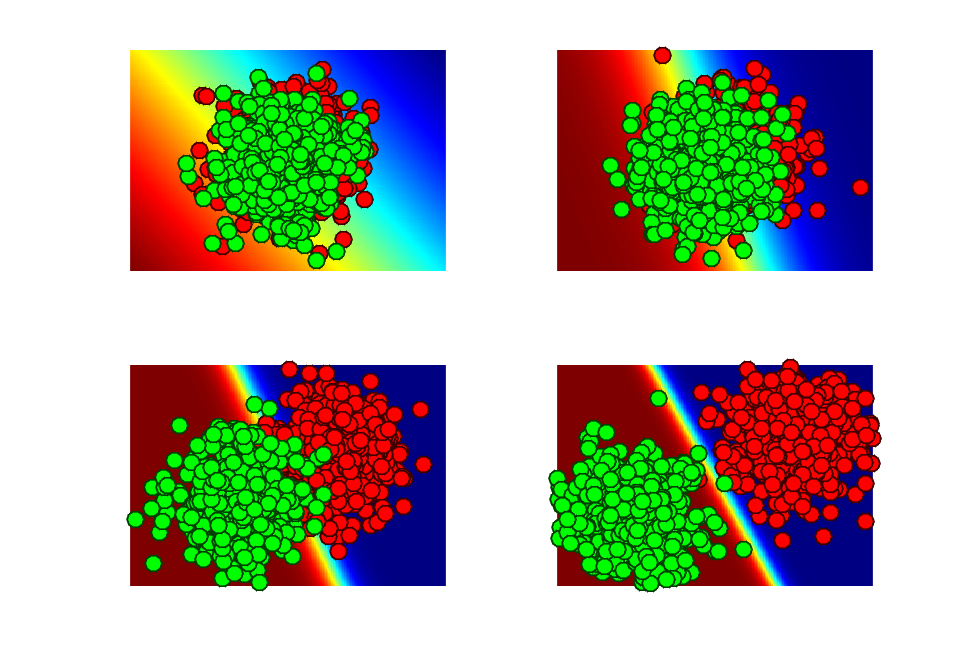
\includegraphics[width=.4\linewidth]{ml/classif/classes-2-separation-influ}
\caption{\label{fig-separation-influ}
Influence on the separation distance between the class on the classification probability. 
}
\end{figure}

To understand the behavior of the method, in Figure~\ref{fig-separation-influ} we generate synthetic data distributed according to a mixture of Gaussian with an overlap governed by an offset $\omega$. 
%
One can display the data overlaid on top of the classification probability, this highlight the separating hyperplane $\enscond{x}{\dotp{\be}{x}=0}$.




%%%%%%%%%%%%%%%%%%%%%%%%%%%%%%%%%%%%%%%%%%%%%%%%%%%%%%%%%%%%
\subsection{Multi-Classes Logistic Classification}
\label{sec-multiclass-logit}

The logistic classification method is extended to an arbitrary number
$k$ of classes by considering a family of weight vectors $\be = ( \be_\ell )_{\ell=1}^k$, which are conveniently stored as columns of a matrix $\be \in \RR^{p \times k}$.

This allows one to model probabilistically the belonging of a point $x \in \RR^p$ to 
the classes using the logit model
\eq{
	 f(x,\be) = \pa{ \frac{ e^{-\dotp{x}{\be_\ell}} }{ \sum_m e^{-\dotp{x}{\be_m}} } }_\ell 
}
This vector $h(x) \in [0,1]^k$ describes the probability of $x$
belonging to the different classes, and $\sum_\ell h(x)_\ell = 1$.

The computation of $\be$ is obtained by solving a maximum likelihood
estimator
 \eq{
	 \umax{\be \in \RR^{p \times k}} \frac{1}{n} \sum_{i=1}^n \log( f(x_i,\be)_{y_i} ) 
}
where we recall that $y_i \in \Yy = \{1,\ldots,k\}$ is the class index of
the point $x_i$.

This is conveniently rewritten as
\eq{
	 \umin{\be \in \RR^{p \times k}} \Ee(\be) \eqdef \sum_i \text{LSE}( X \be )_i - \dotp{X \be}{D} 
}
where $D \in \{0,1\}^{n \times k}$ is the binary class index matrices
\eq{
	  D_{i,\ell} = \choice{
          1 \qifq y_i=\ell, \\
          0 \text{otherwise}.
      }
}
and LSE is the log-sum-exp operator
\eq{
	 \text{LSE}(S) = \log\pa{ \sum_\ell \exp(S_{i,\ell}) } \in \RR^n. 
}
Note that in the case of $k=2$ classes $\Yy=\{-1,1\}$, this model can be shown to be equivalent to the two-classes logistic classifications methods exposed in Section~\eqref{sec-two-class-logit}, with a solution vector being equal to $\be_1-\be_2$ (so it is computationally more efficient to only consider a single vector as we did).

The computation of the LSE operator is
unstable for large value of $S_{i,\ell}$ (numerical overflow, producing NaN), but this can be
fixed by subtracting the largest element in each row,
since 
\eq{
	\text{LSE}(S+a)=\text{LSE}(S)+a
} 
if $a$ is constant along the rows. This is often referred to as  the ``LSE trick'' and is very important to use in practice (in particular if some classes are well separated, since the corresponding $\be_\ell$ vector might become large).


The gradient of the LSE operator is the soft-max operator
\eq{
	  \nabla \text{LSE}(S) = \text{SM}(S) \eqdef
      \pa{
          \frac{
                  e^{S_{i,\ell}}
              }{
                  \sum_m e^{S_{i,m}}
              } }   
}
Similarly to the LSE, it needs to be stabilized by subtracting the maximum value along rows before computation.

\begin{figure}
\centering
\begin{tabular}{@{}c@{\hspace{5mm}}c@{\hspace{5mm}}c@{}}
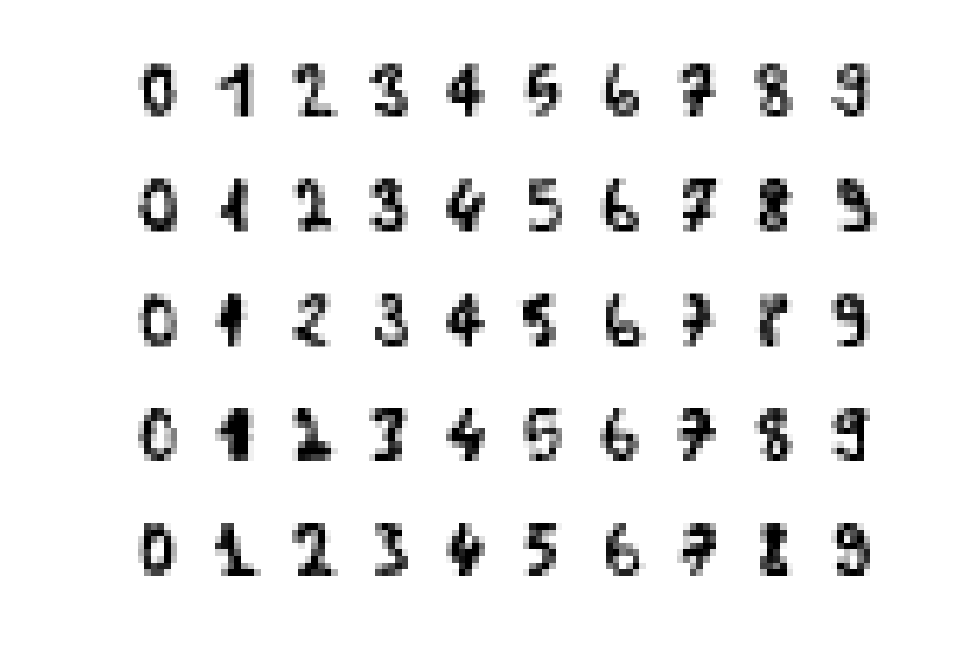
\includegraphics[width=.25\linewidth]{ml/classif/digits}&
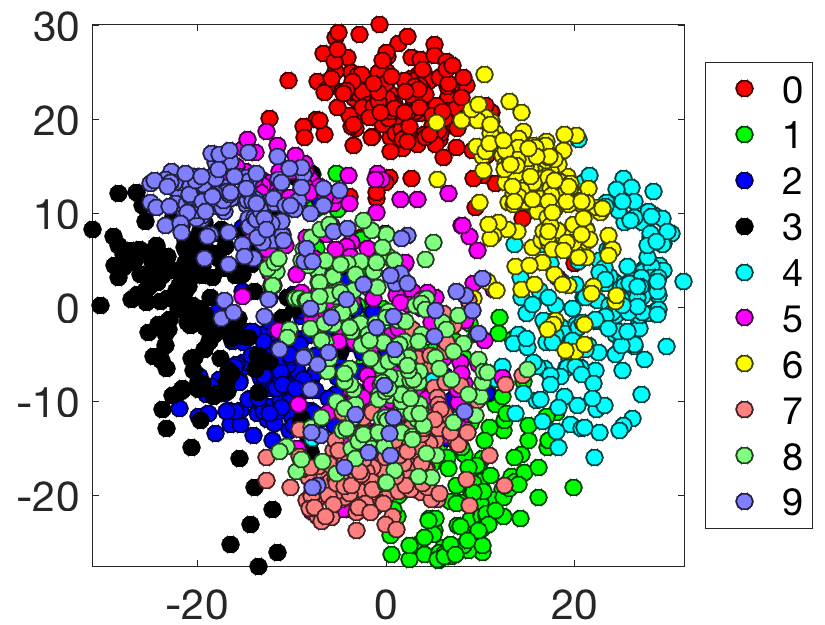
\includegraphics[width=.25\linewidth]{ml/classif/digits-2d}&
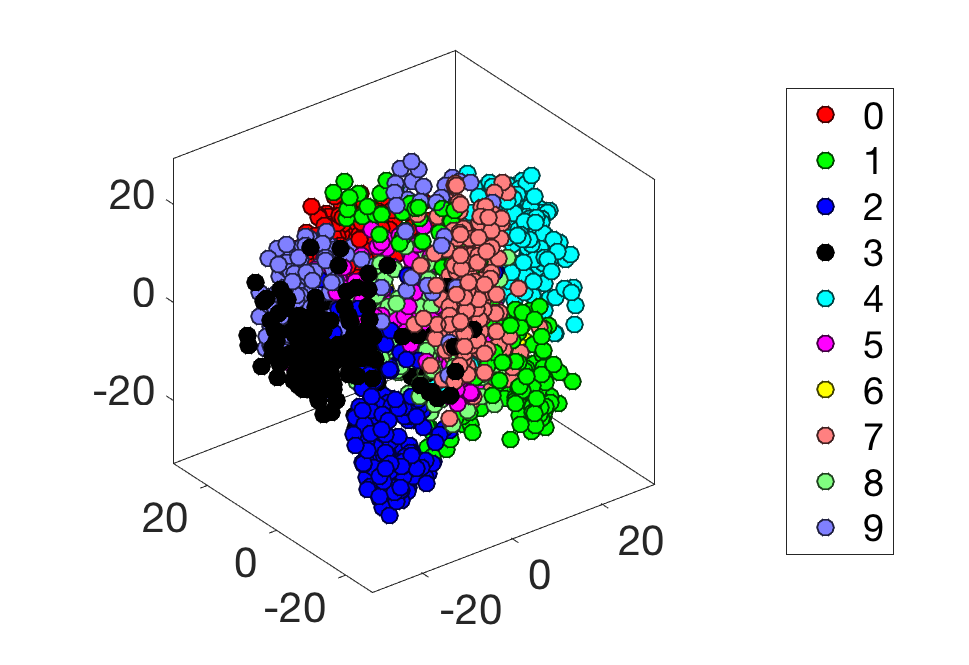
\includegraphics[width=.25\linewidth]{ml/classif/digits-3d}
\end{tabular}
\caption{\label{fig-digits}
2-D and 3-D PCA vizualization of the digits images.
}
\end{figure}

Once $D$ matrix is computed, the gradient of $\Ee$ is computed as 
\eq{
	 \nabla \Ee(\be) =  \frac{1}{n} X^* ( \text{SM}(X \be) - D ).  
}
and one can minimize $\Ee$ using for instance a gradient descent scheme.

To illustrate the method, we use a dataset of $n$ images of size $p = 8 \times 8$, representing digits from 0
to 9 (so there are $k=10$ classes).
%
Figure~\ref{fig-digits} displays a few representative examples as well as 2-D and 3-D PCA projections.
%
Figure~\eqref{fig-digits-classes} displays the ``fuzzy'' decision boundaries by vizualizing the value of $h(x)$ using colors on an image regular grid.

\begin{figure}
\centering
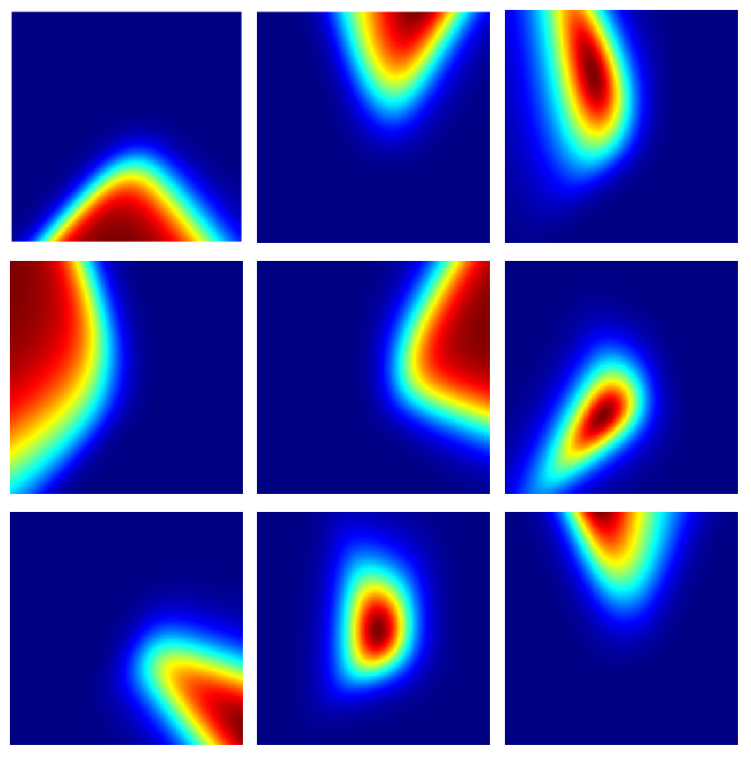
\includegraphics[width=.35\linewidth]{ml/classif/digits-classes}
\qquad
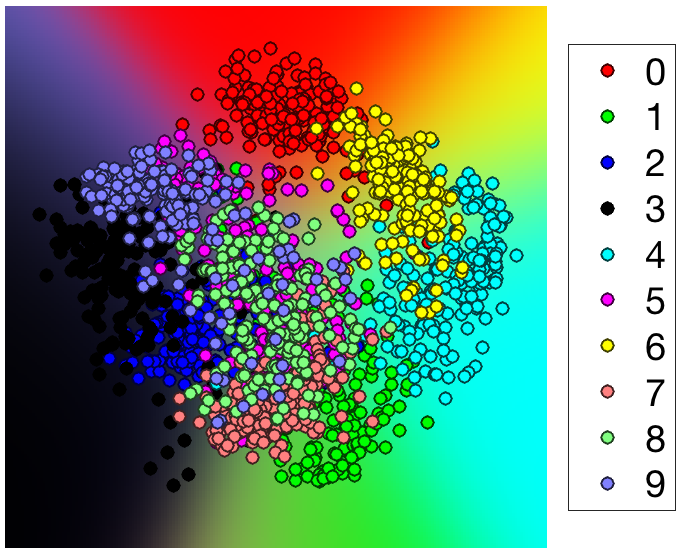
\includegraphics[width=.44\linewidth]{ml/classif/digits-classes-single}
\caption{\label{fig-digits-classes}
Results of digit classification
Left: probability $h(x)_\ell$ of belonging to each of the 9 first classes (displayed over a 2-D PCA space).
Right: colors reflect probability $h(x)$ of belonging to classes.
}
\end{figure}




%%%%%%%%%%%%%%%%%%%%%%%%%%%%%%%%%%%%%%%%%%%%%%%%%%
%%%%%%%%%%%%%%%%%%%%%%%%%%%%%%%%%%%%%%%%%%%%%%%%%%
%%%%%%%%%%%%%%%%%%%%%%%%%%%%%%%%%%%%%%%%%%%%%%%%%%
\section{Kernel Methods}
\label{sec-kernel-methods}

Linear methods are parametric and cannot generate complex regression or decision functions. The linearity assumption is often too restrictive and in some case the geometry of the input functions or classes is not well capture by these models.  In many cases (e.g. for text data) the input data is not even in a linear space, so one cannot even apply these model.

Kernel method is a simple yet surprisingly powerful remedy for these issues. By lifting the features to a high dimensional embedding space, it allows to generate non-linear decision and regression functions, but still re-use the machinery (linear system solvers or convex  optimization algorithm) of linear models. Also, by the use of the so-called ``kernel-trick'', the computation cost does not depends on the dimension of the embedding space, but of the number $n$ of points. It is the perfect example of so-called ``non-parametric'' methods, where the number of degrees of freedom (number of variables involved when fitting the model) grows with the number of samples. This is often desirable when one wants the precisions of the result to improve with $n$, and also to mathematically model the data using ``continuous''  models (e.g. functional spaces such as Sobolev).

The general rule of thumb is that any machine learning algorithm which only makes use of inner products (and not directly of the features $x_i$ themselves) can be ``kernelized'' to obtain a non-parametric algorithm. This is for instance the case for linear and nearest neighbor regression, SVM classification, logistic classification and PCA dimensionality reduction. We first explain the general machinery, and instantiate this in two representative setup (ridge regression, nearest-neighbor regression and logistic classification)

%%%%%%%%%%%%%%%%%%%%%%%%%%%%%%%%%%%%%%%%%%%%%%%%%%
\subsection{Reproducing Kernel Hilbert Space}

We consider a general lifting $\phi : x \in \RR^p \rightarrow \bar x = \phi(x) \in \Hh$ where $\Hh$ is a Hilbert space. 
%
A typical example of lift for $1-D$ values $p=1$ is $\phi(x) = (1,x,x^2,\ldots,x^k) \in \RR^k$ to perform polynomial regression (this can be extended to any dimension $p$ using higher dimensional polynomials).
%
We denote $\bar X = ( \bar x_i^* \eqdef \phi(x_i)^* )_{i=1}^n$ the ``matrix'' where each row is a lifted feature $\phi(x_i)$. For instance, if $\Hh=\RR^{\bar p}$ is finite dimensional, one can view this as a matrix $\bar X \in \RR^{n \times \bar p}$, but the rows of the matrix can be infinite dimensional vectors.

The following proposition is the crux of the RKHS approaches. When using a regularization which is a squared Euclidean norm, $\norm{\cdot}_\Hh^2$, it states that the solutions actually belongs to a data-driven linear sub-space of dimension $n$. Although the proof is straightforward, its implications are very profound, since it leads to tractable algorithms even when using an infinite dimensional lifting space $\Hh$. as we elaborate next. It is often called the ``representer'' theorem in RKHS theory. 

\begin{prop}
	The solution $\be^\star \in \Hh$ of
	\eql{\label{eq-kernel-generic}
		\umin{\be \in \Hh} \Loss(\bar X \be,y) + \frac{\la}{2} \norm{\be}_\Hh^2
	}
	is unique and can be written as
	\eql{\label{eq-rkhs-representer}
		\be = \bar X^* q^\star = \sum_i q_i^\star \phi(x_i) \in \Hh
	}
	where $q \in \RR^N$ is a solution of
	\eql{\label{eq-rkhs-variational}
		\umin{q \in \RR^N} \Loss(K p,y) + \frac{\la}{2} \dotp{K q}{q}_{\RR^n}
	}
	where we defined 
	\eq{
		K \eqdef  \bar X^* \bar X = ( \dotp{\phi(x_i)}{\phi(x_j)}_\Hh )_{i,j=1}^n \in \RR^{n \times n}.
	}
\end{prop}

\begin{proof}
	The first order condition of~\eqref{eq-kernel-generic} reads
	\eq{
		0 \in \bar X^* \partial \Loss(\bar X^* \be^\star,y) + \la \be^\star = 0
	}
	i.e. there exists $u^\star \in \partial \Loss(\bar X^* \be^\star,y)$ such that 
	\eq{
		\be^\star = -\frac{1}{\la} \bar X^* u^\star \in \Im(\bar X^*)
	}
	which is the desired result. 
\end{proof} 

Equation~\eqref{eq-rkhs-representer} expresses the fact that the solution only lives in the $n$ dimensional space spanned by the lifted observed points $\phi(x_i)$.
%
A crucial by product of this results is that all the computations as well as the prediction procedure can be expressed using the so-called kernel $\kappa : \Xx \times \Xx \rightarrow \RR$ associated to $\phi$
\eq{
	\foralls (x,x') \in \Xx^2, \quad \kappa(x,x') \eqdef \dotp{\phi(x')}{\phi(x')}_\Hh.
}
Indeed, one has $K = (\kappa(x_i,x_j))_{i,j}$ and the prediction operator, as a function of $x$ and not $\phi(x)$ (which makes it non-linear) is a weighted sum of kernel functions centered at the $x_i$
\eql{\label{eq-kernel-interp}
	\dotp{\bar x}{\be^\star}_\Hh = \sum_{i=1}^n p_i^\star \dotp{\phi(x)}{\phi(x_i)}_\Hh = \sum_{i=1}^n p_i^\star \kappa(x_i,x).
}
This means that one actually never needs to manipulate quantities in $\Hh$ (which can be infinite dimensional).

But more importantly, one can reverse the process, and instead of starting from a lifting $\phi$, directly consider a kernel $\kappa(x,x')$. This is actually the way this is done in practice, since it is easier to design kernel and think in term of their geometrical properties (for instance, one can sum kernels). In order for this to make sense, the kernel needs to be positive definite, i.e. one should have that $(\kappa(x_i,x_j))_{i,j}$ should be symmetric positive definite for any choice of sampling points $(x_i)_i$. This can be shown to be equivalent to the existence of a lifting function $\phi$ generating the kernel.
%
Note that such a kernel can be defined on arbitrary space (not necessarily Euclidean). 


When using the linear kernel $\kappa(x,y)=\dotp{x}{y}$, one retrieves the linear models studied in the previous section, and the lifting is trivial $\phi(x)=x$.
%
A family of popular kernels are polynomial ones,  $\kappa(x,x') = (\dotp{x}{y}+c)^a$ for $a
\in \NN^*$ and $c>0$, which corresponds to a lifting in finite dimension. For instance, for $a=2$ and $p=2$, one has a lifting in dimension $6$
\eq{
	\kappa(x,x') = \pa{ x_1 x_1' + x_1 x_1' + c}^2 = \dotp{\phi(x)}{\phi(x')}
	\qwhereq
	\phi(x)=(x_1^2,x_2^2,\sqrt{2}x_1x_2,\sqrt{2c}x_1,\sqrt{2c}x_2,c)^* \in \RR^6.	
}

In Euclidean spaces, the gaussian kernel is the most well known and used kernel
\eql{\label{eq-gauss-kernel}
	 \kappa(x,y) \eqdef e^{-\frac{\norm{x-y}^2}{2\sigma^2}} . 
}
The bandwidth parameter $\si>0$ is crucial and controls the locality of
the model. It is typically tuned through cross validation. It corresponds to an infinite dimensional lifting $x \mapsto e^{-\frac{\norm{x-\cdot}^2}{2(\sigma/2)^2}} \in L^2(\RR^p)$.
%
Another related popular kernel is the Laplacian kernel $\exp(-\norm{x-y}/\si)$.
%
More generally, when considering translation invariant kernels $\kappa(x,x') = k(x-x')$ on $\RR^p$, being positive definite is equivalent to $\hat k(\om)>0$ where $\hat k$ is the Fourier transform, and the associated lifting is obtained by considering $\hat h=\sqrt{\hat \kappa}$ and $\phi(x)=h(x-\cdot) \in L^2(\RR^p)$. 

%%%%%%%%%%%%%%%%%%%%%%%%%%%%%%%%%%%%%%%%%%%%%%%%%%
\subsection{Examples of Kernelized Algorithms}

We illustrate this general machinery by applying it to three typical problems. 

%%
\paragraph{Kernelized ridge regression.}

The simplest instantiation of this kernelization approach is when using the square loss $L(y,y')=\frac{1}{2}|y-y'|^2$, which is the ridge regression problem studied in Section~\ref{sec-linear-models}. The obtain regression model~\eqref{eq-kernel-interp} corresponds to approximating the data using a weighted sum of data-centered kernel function $\kappa(x_i,\cdot)$. When using a Gaussian kernel~\eqref{eq-gauss-kernel}, the bandwidth $\si$ controls the smoothness of the approximation. This is illustrated in Figure~\ref{fig-kernel}. 


\begin{figure}
\centering
\begin{tabular}{@{}c@{\hspace{1mm}}c@{\hspace{1mm}}c@{\hspace{1mm}}c@{\hspace{1mm}}c@{}}
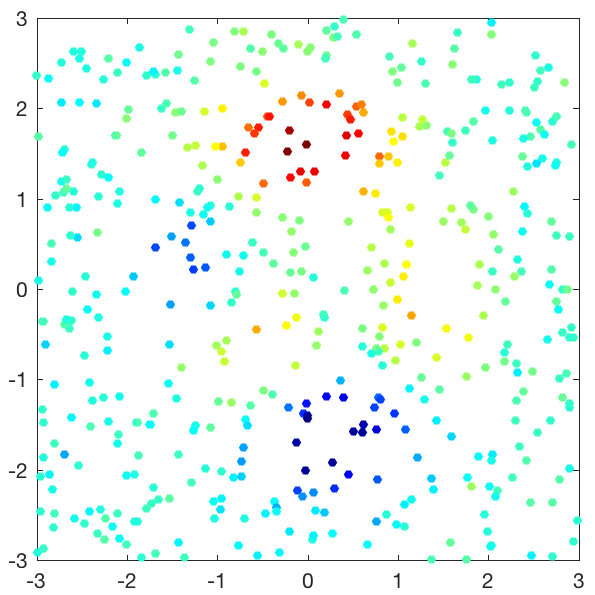
\includegraphics[width=.19\linewidth]{ml/regression/scatter-2d}&
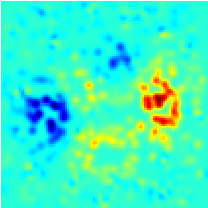
\includegraphics[width=.19\linewidth]{ml/regression/kernel-2}&
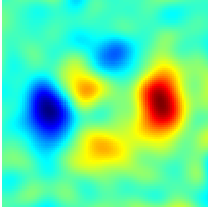
\includegraphics[width=.19\linewidth]{ml/regression/kernel-3}&
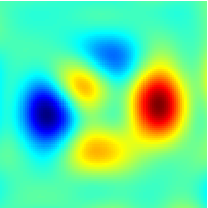
\includegraphics[width=.19\linewidth]{ml/regression/kernel-4}&
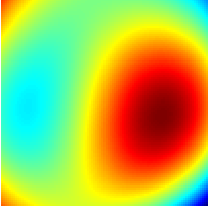
\includegraphics[width=.19\linewidth]{ml/regression/kernel-5}\\
& $\si=0.1$ & $\si=0.5$ & $\si=1$ & $\si=5$
\end{tabular}
\caption{\label{fig-kernel}
Regression using a Gaussian kernel.
}
\end{figure}


In this special case of a square loss, one can solve in closed form~\eqref{eq-rkhs-variational} by solving a $n \times n$ linear system
\eq{
	q^\star = (K K+\la K)^{-1} K y =  (K+\la \Id_N)^{-1} y
}
This expression matches exactly~\eqref{eq-linest-woodbury} when using $K$ in place of $\hat C$

%%%
\paragraph{Kernelized logistic classification.}

Logistic classification tries to separate the classes using a linear separating hyperplane $\enscond{x}{\dotp{\be}{x}=0}$. 
%
In order to generate a non-linear decision boundary, one can replace the parametric linear model by a non-linear non-parametric model, thanks to kernelization.  This allows in particular to generate decision boundaries of arbitrary complexity.

In the two class problem, as detailed in Section~\ref{sec-two-class-logit}, one solves~\eqref{eq-rkhs-variational} using the logistic loss~\eqref{eq-logistic-loss}. This can be for instance achieved by a gradient descent method.
%
Once the solution $q^\star$ is obtained, the probability of $x$ belonging to the first class is then
\eq{
	\th( \sum_{i=1}^n q_i^\star \kappa(x_i,x) ).
} 
Figure~\ref{fig-classes-kernel} illustrate such a non-linear decision function on a simple 2-D problem.


\begin{figure}
\centering
\begin{tabular}{@{}c@{\hspace{5mm}}c@{}}
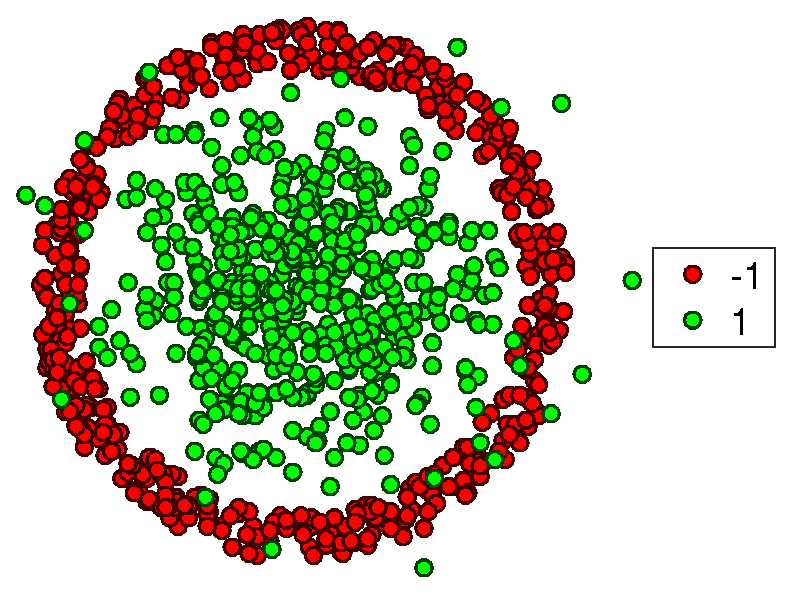
\includegraphics[width=.35\linewidth]{ml/classif/classes-kernel}&
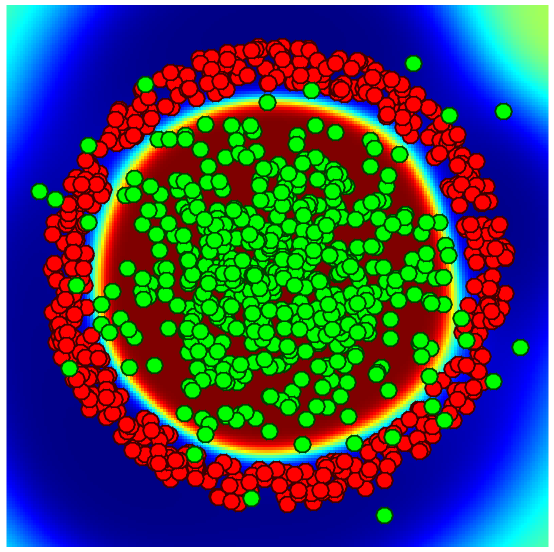
\includegraphics[width=.25\linewidth]{ml/classif/classes-kernel-result}
\end{tabular}
\caption{\label{fig-classes-kernel}
Non-linear classification using a Gaussian kernel.
}
\end{figure}


%%
\paragraph{Kernelized nearest-neihbors. }

It is also possible to extend nearest neighbor classification (as detailed in Section~\ref{sec-nn-classif}) and regression over a lifted space by making use only of kernel evaluation, simply noticing that
\eq{
	\norm{\phi(x_i)-\phi(x_j)}_\Hh^2 = \kappa(x_i,x_i)+\kappa(x_j,x_j) - 2 \kappa(x_i,x_j).	
}


%%
\paragraph{Kernel on strings. }

\todo{write me}


